\documentclass{beamer}\usepackage[]{graphicx}\usepackage[]{color}
% maxwidth is the original width if it is less than linewidth
% otherwise use linewidth (to make sure the graphics do not exceed the margin)
\makeatletter
\def\maxwidth{ %
  \ifdim\Gin@nat@width>\linewidth
    \linewidth
  \else
    \Gin@nat@width
  \fi
}
\makeatother

\definecolor{fgcolor}{rgb}{0.345, 0.345, 0.345}
\newcommand{\hlnum}[1]{\textcolor[rgb]{0.686,0.059,0.569}{#1}}%
\newcommand{\hlstr}[1]{\textcolor[rgb]{0.192,0.494,0.8}{#1}}%
\newcommand{\hlcom}[1]{\textcolor[rgb]{0.678,0.584,0.686}{\textit{#1}}}%
\newcommand{\hlopt}[1]{\textcolor[rgb]{0,0,0}{#1}}%
\newcommand{\hlstd}[1]{\textcolor[rgb]{0.345,0.345,0.345}{#1}}%
\newcommand{\hlkwa}[1]{\textcolor[rgb]{0.161,0.373,0.58}{\textbf{#1}}}%
\newcommand{\hlkwb}[1]{\textcolor[rgb]{0.69,0.353,0.396}{#1}}%
\newcommand{\hlkwc}[1]{\textcolor[rgb]{0.333,0.667,0.333}{#1}}%
\newcommand{\hlkwd}[1]{\textcolor[rgb]{0.737,0.353,0.396}{\textbf{#1}}}%
\let\hlipl\hlkwb

\usepackage{framed}
\makeatletter
\newenvironment{kframe}{%
 \def\at@end@of@kframe{}%
 \ifinner\ifhmode%
  \def\at@end@of@kframe{\end{minipage}}%
  \begin{minipage}{\columnwidth}%
 \fi\fi%
 \def\FrameCommand##1{\hskip\@totalleftmargin \hskip-\fboxsep
 \colorbox{shadecolor}{##1}\hskip-\fboxsep
     % There is no \\@totalrightmargin, so:
     \hskip-\linewidth \hskip-\@totalleftmargin \hskip\columnwidth}%
 \MakeFramed {\advance\hsize-\width
   \@totalleftmargin\z@ \linewidth\hsize
   \@setminipage}}%
 {\par\unskip\endMakeFramed%
 \at@end@of@kframe}
\makeatother

\definecolor{shadecolor}{rgb}{.97, .97, .97}
\definecolor{messagecolor}{rgb}{0, 0, 0}
\definecolor{warningcolor}{rgb}{1, 0, 1}
\definecolor{errorcolor}{rgb}{1, 0, 0}
\newenvironment{knitrout}{}{} % an empty environment to be redefined in TeX

\usepackage{alltt}

\usepackage{animate}

\def\currentCourse{Unsupervised Learning}
\def\currentInstitute{MAP 573, 2019 -- Julien Chiquet}
\def\currentLogo{../common_figs/logo_X}
\def\currentDate{\'Ecole Polytechnique, Autumn semester, 2019}
\def\currentChapter{Introduction to clustering}


% THEME BEAMER
\usepackage{../beamer_theme}

\graphicspath{{figures/},{../common_figs/}}

\usepackage{multirow}
\usepackage{tikz}
\usepackage[vlined]{algorithm2e}

\pgfdeclareimage[width=.5cm]{computer}{computer.png}

% \usetikzlibrary{calc,shapes,backgrounds,arrows,automata,shadows,positioning}
% \tikzstyle{every state}=[fill=red,draw=none,scale=0.7,font=\small,text=white]
% \tikzstyle{every edge}=[-,shorten >=1pt,auto,thin,draw]
% \tikzstyle{alertstate}=[fill=bleu]
% \definecolor{genecolor}{RGB}{94,135,173}

\title{\currentCourse}

\subtitle{\huge\currentChapter\normalsize}

\institute{\currentInstitute}

\date{\currentDate}



\AtBeginSection{
  \begin{frame}<beamer>
    \frametitle{Outline}
    \framesubtitle{\insertpart}
    \tableofcontents[currentsection,currentsubsection, subsectionstyle=show/shaded/hide]  
  \end{frame}
}

\AtBeginSubsection{
  \begin{frame}<beamer>
    \frametitle{Outline}
    \framesubtitle{\insertpart}
    \tableofcontents[currentsection,currentsubsection, subsectionstyle=show/shaded/hide]  
  \end{frame}
}

\AtBeginSubsubsection{
  \begin{frame}<beamer>
    \frametitle{Outline}
    \framesubtitle{\insertpart}
    \tableofcontents[currentsection,currentsubsection, subsectionstyle=show/shaded/hide]  
  \end{frame}
}

\newcommand{\dotitlepage}{%
  \begin{frame}
    \titlepage
    \vfill
    \begin{center}
        \scriptsize\url{https://github.com/jchiquet/CourseUnsupervisedLearningX}
    \end{center}
    \vfill
    \includegraphics[width=2cm]{\currentLogo}\hfill
    
\includegraphics[width=2.5cm]{logo_inra}
  \end{frame}
  %
}

\newcommand{\dotoc}{%
  \begin{frame}
    \frametitle{Outline}
    \tableofcontents[currentsection,
    sectionstyle=show/show,
    subsectionstyle=hide]
  \end{frame}
  %
}

\usetikzlibrary{calc,shapes,backgrounds,arrows,automata,shadows,positioning}
\IfFileExists{upquote.sty}{\usepackage{upquote}}{}
\begin{document}

\dotitlepage

\begin{frame}
	\frametitle{Machine Learning}

	\begin{center}
		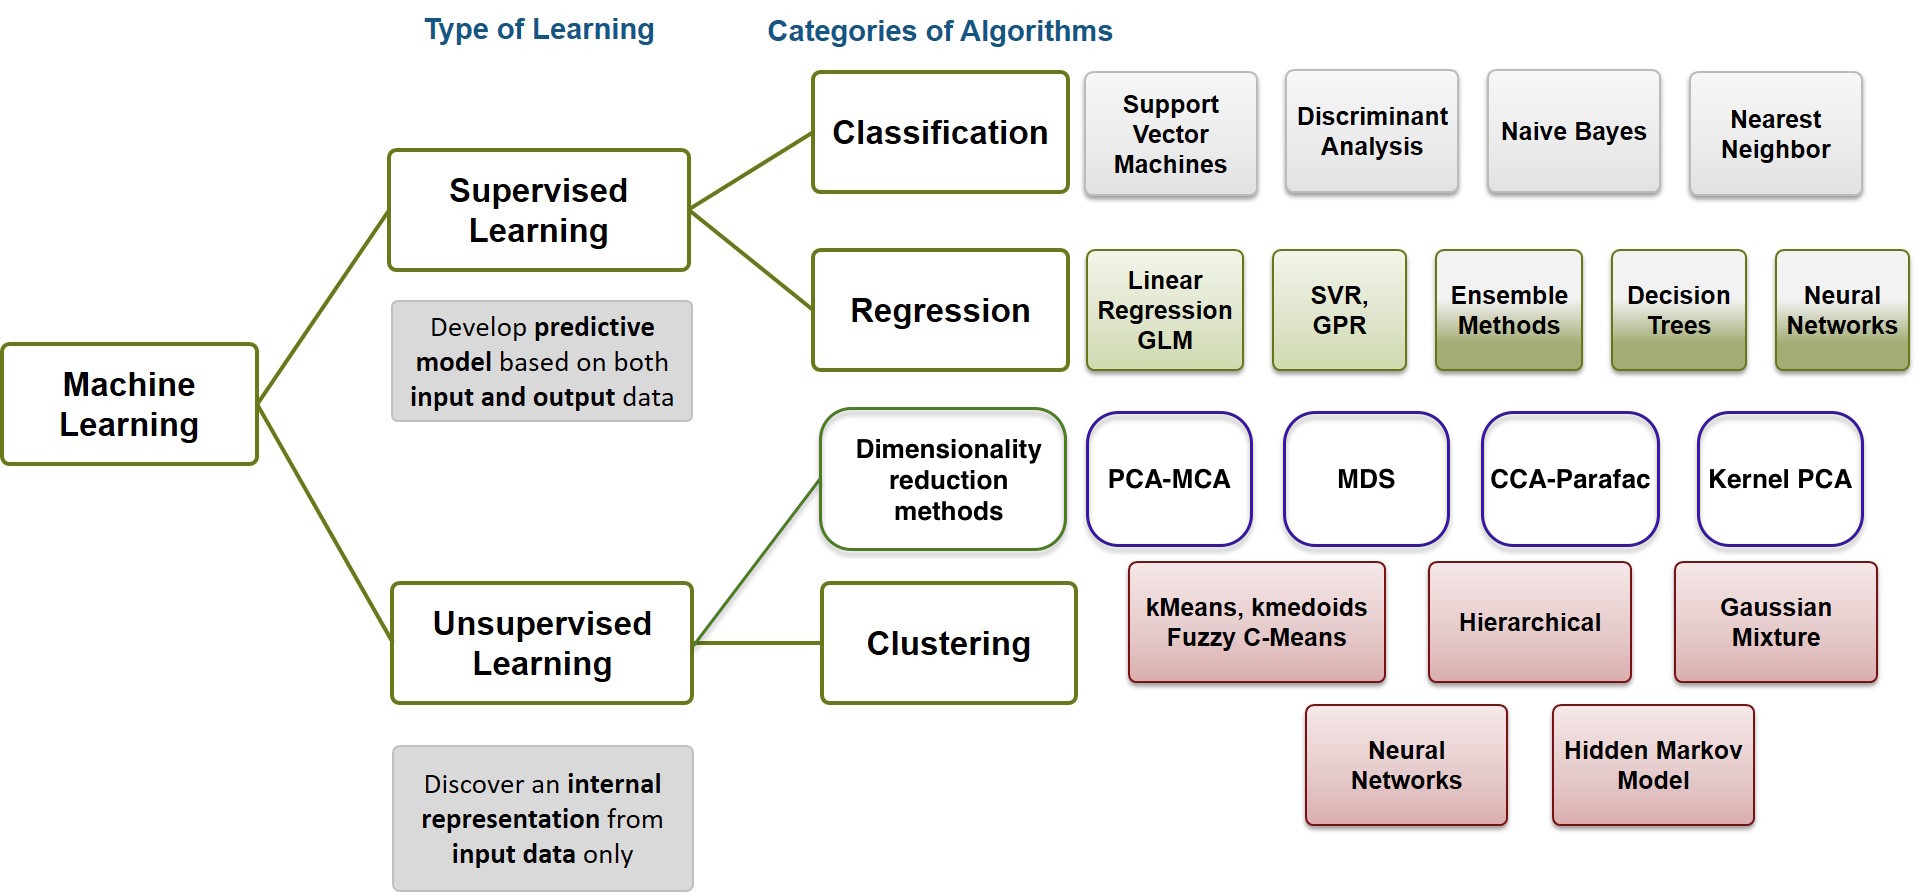
\includegraphics[width=\textwidth]{figures/Learning+Types.jpg}
	\end{center}

\end{frame}

\begin{frame}
  \frametitle{Supervised vs Unsupervised Learning}
  
  \begin{block}{Supervised Learning}
    \begin{itemize}
    \item Training data $\mathcal{D}_n = \{(\bx_1, y_1), \ldots, (\bx_n, y_n)\}, X_i \sim^{\text{i.i.d}} \mathbb{P}$
    \item Construct a predictor $\hat f : \mathcal{X} \rightarrow \mathcal{Y}$ using $\mathcal{D}_n$
    \item Loss $\ell(y, f(x))$ measures how well $f(x)$ predicts $y$
    \item Aim: minimize the generalization error
    \item Task: Regression, Classification
    \end{itemize}
    $\rightsquigarrow$ The goal is clear: predict $y$ based on $x$ (regression, classification)
  \end{block}

  \begin{block}{Unsupervised Learning}
  \begin{itemize}
    \item Training data $\mathcal{D} = \{\bx_1, \ldots, \bx_n\}$
    \item Loss? , Aim?
    \item Task: Dimension reduction, Clustering
  \end{itemize}  
  $\rightsquigarrow$ The goal is less well defined, and \emph{validation} is questionable
  \end{block}
  
\end{frame}

\begin{frame}
  \frametitle{Outline}
  \tableofcontents
\end{frame}

%% ==========================================================================
\section{Clustering: introduction}
%% ==========================================================================

\begin{frame}[fragile]
  \frametitle{Packages required for reproducing the slides}
  
\begin{knitrout}\scriptsize
\definecolor{shadecolor}{rgb}{0.969, 0.969, 0.969}\color{fgcolor}\begin{kframe}
\begin{alltt}
\hlkwd{library}\hlstd{(tidyverse)}  \hlcom{# opinionated collection of packages for data manipulation}
\hlkwd{library}\hlstd{(corrplot)}   \hlcom{# fancy plots of matrices as images}
\hlkwd{library}\hlstd{(GGally)}     \hlcom{# extension to ggplot vizualization system}
\hlkwd{library}\hlstd{(ggfortify)}  \hlcom{# extension to ggplot vizualization system}
\hlkwd{library}\hlstd{(mclust)}     \hlcom{# Gaussian mixture models}
\hlkwd{library}\hlstd{(aricode)}    \hlcom{# fast computation of clustering measures}
\hlkwd{library}\hlstd{(animation)}  \hlcom{# kmeans animation slides}
\hlcom{# color and plots themes}
\hlkwd{library}\hlstd{(RColorBrewer)}
\hlstd{pal} \hlkwb{<-} \hlkwd{brewer.pal}\hlstd{(}\hlnum{10}\hlstd{,} \hlstr{"Set3"}\hlstd{)}
\hlkwd{theme_set}\hlstd{(}\hlkwd{theme_bw}\hlstd{())}
\end{alltt}
\end{kframe}
\end{knitrout}
  
\end{frame}

\subsection{Motivating example}

\begin{frame}[fragile]
  \frametitle{Companion data set}
  \framesubtitle{Morphological Measurements on Leptograpsus Crabs}
  
\begin{block}{Description}
\small The crabs data frame has 200 rows and 8 columns, describing 5 morphological measurements on 50 crabs each of two colour forms and both sexes, of the species \textit{Leptograpsus variegatus} collected at Fremantle, W. Australia.
\end{block}
  
\begin{knitrout}\scriptsize
\definecolor{shadecolor}{rgb}{0.969, 0.969, 0.969}\color{fgcolor}\begin{kframe}
\begin{alltt}
\hlstd{crabs} \hlkwb{<-} \hlstd{MASS}\hlopt{::}\hlstd{crabs} \hlopt \hlkwd{select}\hlstd{(}\hlopt{-}\hlstd{index)} \hlopt
  \hlkwd{rename}\hlstd{(}\hlkwc{sex} \hlstd{= sex,}
         \hlkwc{species}         \hlstd{= sp,}
         \hlkwc{frontal_lob}     \hlstd{= FL,}
         \hlkwc{rear_width}      \hlstd{= RW,}
         \hlkwc{carapace_length} \hlstd{= CL,}
         \hlkwc{carapace_width}  \hlstd{= CW,}
         \hlkwc{body_depth}      \hlstd{= BD)}
\hlstd{crabs} \hlopt \hlkwd{select}\hlstd{(sex, species)} \hlopt \hlkwd{summary}\hlstd{()} \hlopt \hlstd{knitr}\hlopt{::}\hlkwd{kable}\hlstd{(}\hlstr{"latex"}\hlstd{)}
\end{alltt}
\end{kframe}
\begin{tabular}{l|l|l}
\hline
  & sex & species\\
\hline
 & F:100 & B:100\\
\hline
 & M:100 & O:100\\
\hline
\end{tabular}


\end{knitrout}
\end{frame}

\begin{frame}[fragile]
  \frametitle{Companion data set II}
  \framesubtitle{Pairs plot of attributes}

\begin{knitrout}\scriptsize
\definecolor{shadecolor}{rgb}{0.969, 0.969, 0.969}\color{fgcolor}\begin{kframe}
\begin{alltt}
\hlkwd{ggpairs}\hlstd{(crabs,} \hlkwc{columns} \hlstd{=} \hlnum{3}\hlopt{:}\hlnum{7}\hlstd{,} \hlkwd{aes}\hlstd{(}\hlkwc{colour} \hlstd{= species,} \hlkwc{shape} \hlstd{= sex))}
\end{alltt}
\end{kframe}
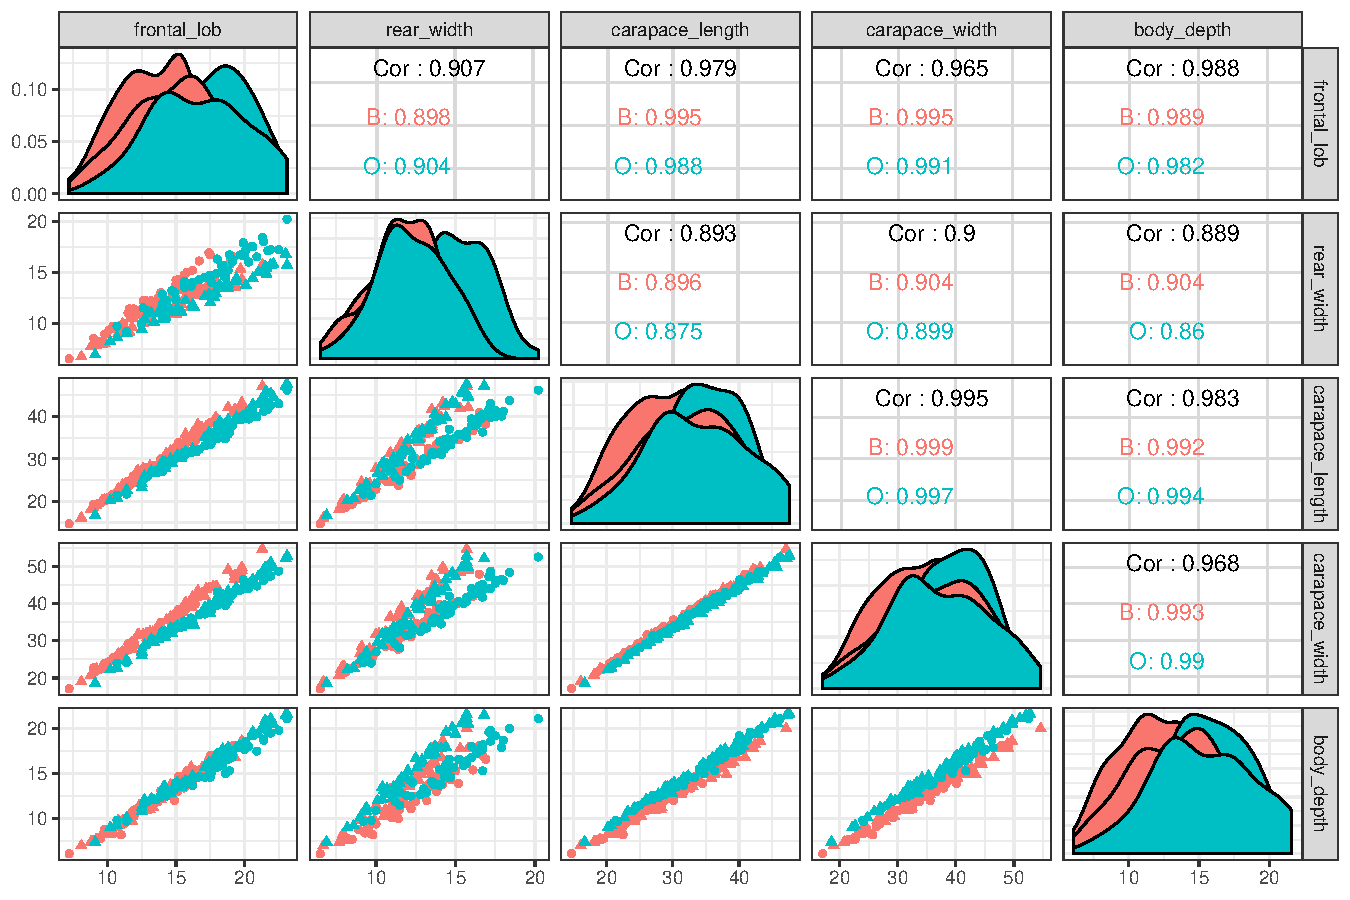
\includegraphics[width=.8\textwidth]{figures/crabs_attributes-1} 

\end{knitrout}
\end{frame}

\begin{frame}[fragile]
  \frametitle{Companion data set III}
  \framesubtitle{PCA on the attributes}

\begin{knitrout}\scriptsize
\definecolor{shadecolor}{rgb}{0.969, 0.969, 0.969}\color{fgcolor}\begin{kframe}
\begin{alltt}
\hlkwd{prcomp}\hlstd{(}\hlkwd{select}\hlstd{(crabs,} \hlopt{-}\hlstd{species,} \hlopt{-}\hlstd{sex),} \hlkwc{scale.} \hlstd{=} \hlnum{TRUE}\hlstd{)} \hlopt
  \hlkwd{autoplot}\hlstd{(}\hlkwc{loadings} \hlstd{=} \hlnum{TRUE}\hlstd{,} \hlkwc{loadings.label} \hlstd{=} \hlnum{TRUE}\hlstd{,}
           \hlkwc{data} \hlstd{= crabs,} \hlkwc{colour} \hlstd{=} \hlstr{'species'}\hlstd{,} \hlkwc{shape} \hlstd{=} \hlstr{'sex'}\hlstd{)}
\end{alltt}
\end{kframe}
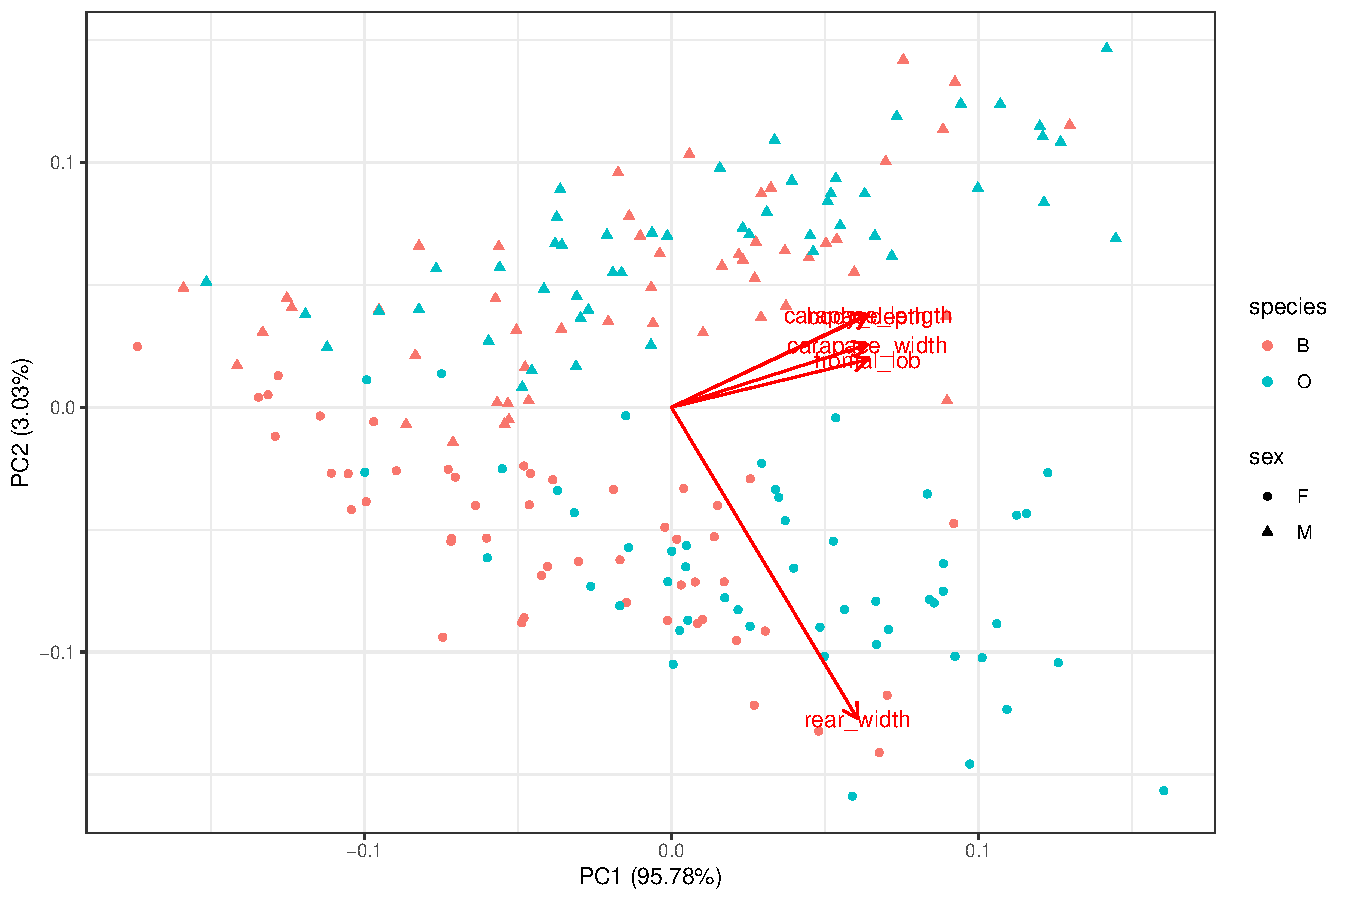
\includegraphics[width=.8\textwidth]{figures/pca_crabs_untransformed-1} 

\end{knitrout}

\end{frame}

\begin{frame}[fragile,allowframebreaks]
  \frametitle{Remove size effect}
  \framesubtitle{Carried by the 1st principal component}

\paragraph{PCA is solved by SVD}
\begin{equation*}
  \mathbf{X} = \mathbf{U} \mathbf{D} \mathbf{V}^\top.
\end{equation*}

We remove the best rank-1 approximation of $\mathbf{X}$ to remove the \textit{size effect}, carried by the first axis, that is,
\begin{equation*}
  \tilde{\mathbf{X}}^{(1)} = \mathbf{U}_{\bullet 1} d_{11} \mathbf{v}_{\bullet 1}^\top.
\end{equation*}


\begin{knitrout}\scriptsize
\definecolor{shadecolor}{rgb}{0.969, 0.969, 0.969}\color{fgcolor}\begin{kframe}
\begin{alltt}
\hlstd{attributes} \hlkwb{<-} \hlkwd{select}\hlstd{(crabs,} \hlopt{-}\hlstd{sex,} \hlopt{-}\hlstd{species)}
\hlstd{SVD} \hlkwb{<-} \hlkwd{svd}\hlstd{(attributes)}
\hlstd{attributes_rank1} \hlkwb{<-} \hlkwd{tcrossprod}\hlstd{(SVD}\hlopt{$}\hlstd{u[,} \hlnum{1}\hlstd{]} \hlopt{*} \hlstd{SVD}\hlopt{$}\hlstd{d[}\hlnum{1}\hlstd{], SVD}\hlopt{$}\hlstd{v[,} \hlnum{1}\hlstd{])}
\hlstd{crabs_corrected} \hlkwb{<-} \hlstd{crabs}
\hlstd{crabs_corrected[,} \hlnum{3}\hlopt{:}\hlnum{7}\hlstd{]} \hlkwb{<-} \hlstd{attributes} \hlopt{-} \hlstd{attributes_rank1}
\end{alltt}
\end{kframe}
\end{knitrout}

$\rightsquigarrow$ Axis 1 explains a latent effect, here the size in the case at hand, common to all attributes.

\begin{knitrout}\scriptsize
\definecolor{shadecolor}{rgb}{0.969, 0.969, 0.969}\color{fgcolor}\begin{kframe}
\begin{alltt}
\hlkwd{ggpairs}\hlstd{(crabs_corrected,} \hlkwc{columns} \hlstd{=} \hlnum{3}\hlopt{:}\hlnum{7}\hlstd{,} \hlkwd{aes}\hlstd{(}\hlkwc{colour} \hlstd{= species,} \hlkwc{shape} \hlstd{= sex))}
\end{alltt}
\end{kframe}
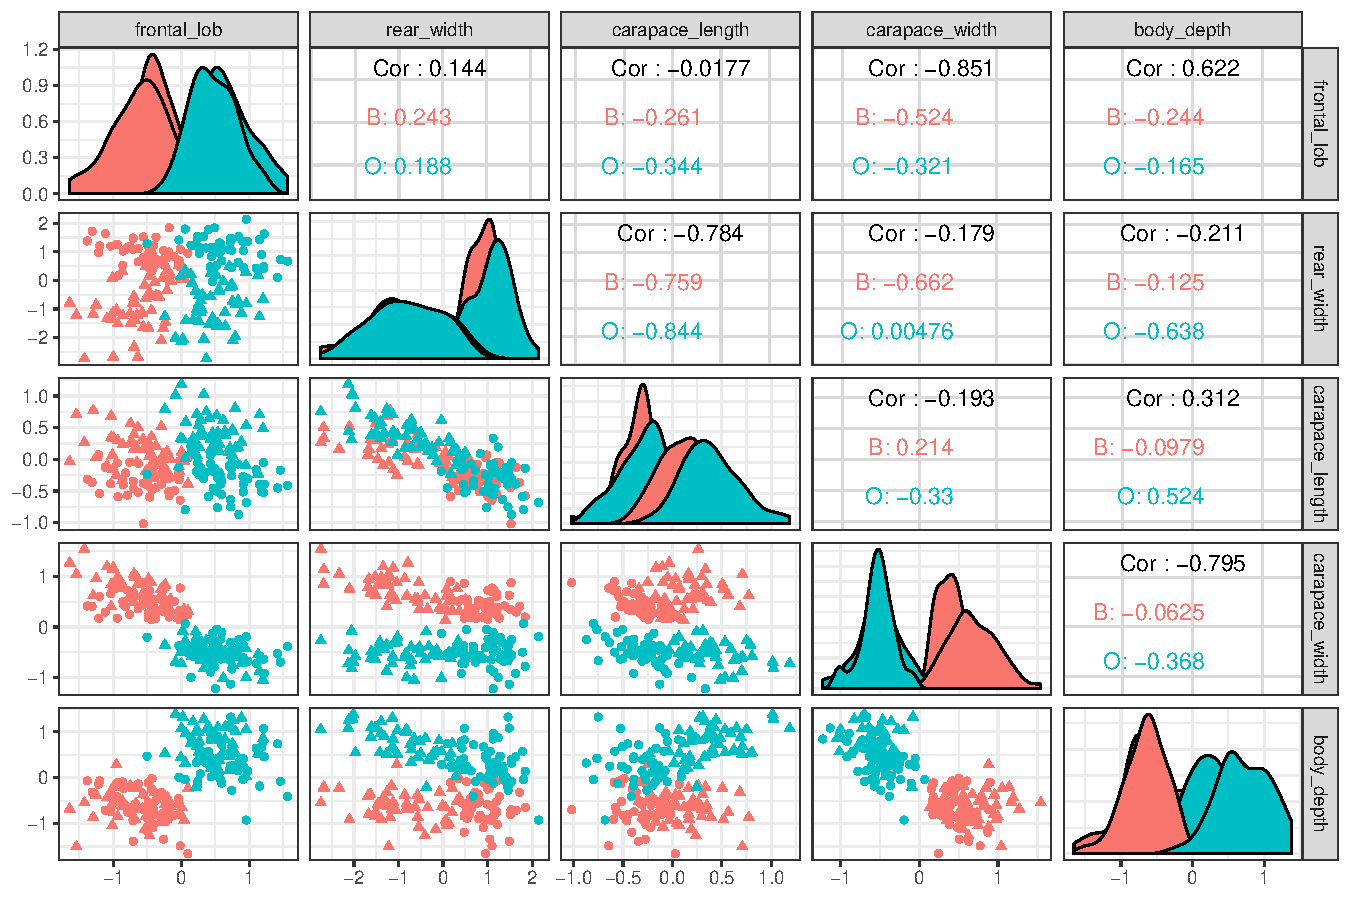
\includegraphics[width=.8\textwidth]{figures/pairs_plot_corrected-1} 

\end{knitrout}

\end{frame}

\begin{frame}[fragile]
  \frametitle{PCA on corrected data}
\begin{knitrout}\scriptsize
\definecolor{shadecolor}{rgb}{0.969, 0.969, 0.969}\color{fgcolor}\begin{kframe}
\begin{alltt}
\hlkwd{prcomp}\hlstd{(}\hlkwd{select}\hlstd{(crabs_corrected,} \hlopt{-}\hlstd{species,} \hlopt{-}\hlstd{sex),} \hlkwc{scale.} \hlstd{=} \hlnum{TRUE}\hlstd{)} \hlopt
  \hlkwd{autoplot}\hlstd{(}\hlkwc{loadings} \hlstd{=} \hlnum{TRUE}\hlstd{,} \hlkwc{loadings.label} \hlstd{=} \hlnum{TRUE}\hlstd{,}
           \hlkwc{data} \hlstd{= crabs_corrected,} \hlkwc{colour} \hlstd{=} \hlstr{'species'}\hlstd{,} \hlkwc{shape} \hlstd{=} \hlstr{'sex'}\hlstd{)}
\end{alltt}
\end{kframe}
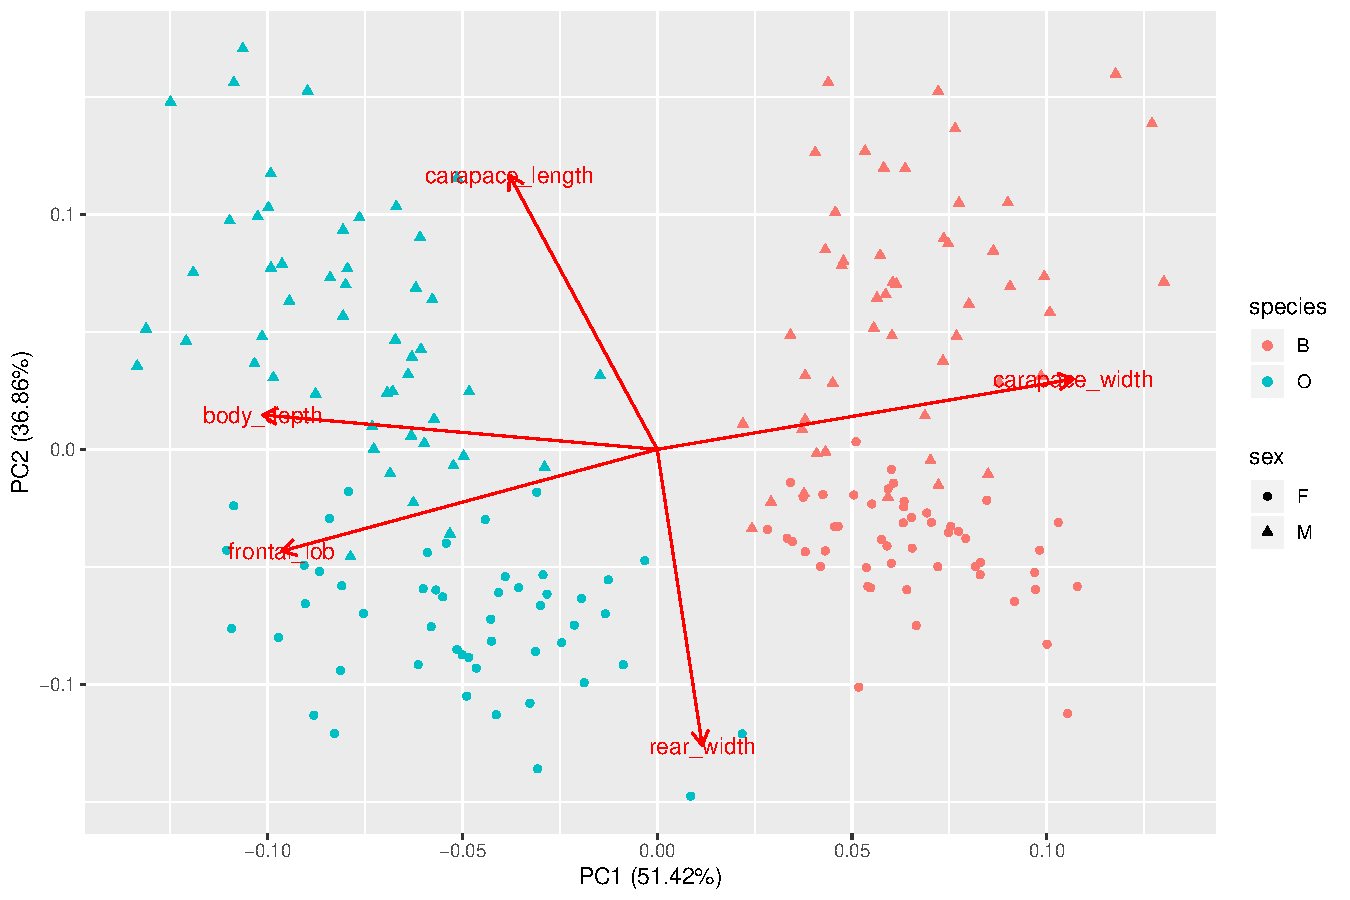
\includegraphics[width=.8\textwidth]{figures/pca_crabs_corrected-1} 

\end{knitrout}
\end{frame}

\begin{frame}
  \frametitle{Questions}
  \begin{center}
    \begin{enumerate}
      \item Could we automatically identify some grouping (\alert{clustering}) between samples ?
      \item Would this clustering correspond to some known labels (sex, species)?
      \item Does it matter?
    \end{enumerate}
  \end{center}

\end{frame}

\subsection{Generalities}

\begin{frame}[label=Clustering1]
  \frametitle{Clustering: general goals}

  \paragraph{Objective}: construct a map $f$ from $\mathcal{D}$ to $\{1,\ldots,K\}$ where $K$ is a fixed number of clusters.
    
  \vfill
    
  \paragraph{Careful! classification $\neq$ clustering}
      \begin{itemize}
      \item Classification presupposes the existence of classes
      \item Clustering labels only elements of the dataset
      \begin{itemize}
      \item[$\rightsquigarrow$] no ground truth (no given labels)
      \item[$\rightsquigarrow$] discovers a structure "natural" to the data
      \item[$\rightsquigarrow$] not necessarily related to a known classification
      \end{itemize}
      \end{itemize}
  
  \vfill

  \paragraph{Motivations}
    \begin{itemize}
    \item describe large masses of data in a simplified way,
    \item structure a set of knowledge,
    \item reveal structures, hidden causes,
    \item use of the groups in further processing, 
    \item \dots
  \end{itemize}

\end{frame}

\begin{frame}[label=Clustering2]

  \frametitle{Clustering: challenges}

    \begin{block}{Clustering quality}
      No obvious measure to define the \alert{quality} of the clusters. Ideas:
      \begin{itemize}
        \item \alert{Inner} homogeneity: samples in the same group should be similar
        \item \alert{Outer} inhomogeneity: samples in different groups should be different
      \end{itemize}
    \end{block}

    \vspace{-.25cm}

    \begin{block}{Number of clusters}
      Choice of the number of clusters $K$ often complex
      \begin{itemize}
        \item No ground truth in unsupervised learning!
        \item Several solutions might be equally good
      \end{itemize}
    \end{block}

    \vspace{-.25cm}

    \begin{block}{Two general approaches}
      \vspace{-.25cm}
      \begin{itemize}
        \item \alert{distance-based}: require a distance/dissimilarity between $\{\bx_i\}$
        \item \alert{model-based}: require assumptions on the distribution $\mathbb{P}$
      \end{itemize}
    \end{block}
    
\end{frame}

\subsection{Vocabulary}

\begin{frame}
  \frametitle{Dissimilarity and Distance}

  \paragraph{\it Clustering requires a measure of ressemblance between object}

  \begin{definition}[(dis)similarity]
    Similarity (\textit{resp. Dissimilarity}) measures the ressemblance (\textit{resp. discrepancy}) between objects based on several features. 
  \end{definition}

  For instance, two objects are similar if 
  \begin{itemize}
    \item they share a certain feature
    \item \alert{their features are close according to a measure of proximity}
  \end{itemize}
  
  \vfill
  
  \begin{definition}[distance/metric]<2>
    Dissimilairty can be measuresd by distances, \textit{i.e.} a function $d_{ij}$ between pairs in \{$\bx_i\}$ s.t.
    \vspace{-.25cm}
    \begin{multicols}{2}
    \begin{itemize}
      \item $d_{ij} \geq 0$,
      \item $d_{ij} = 0 \Leftrightarrow \bx_i = \bx_{j}$,
      \item $d_{ij} = d_{ji}$,
      \item $d_{ik} \leq d_{ij} + d_{jk}$.
    \end{itemize}
    \end{multicols}
  \end{definition}

\end{frame}

\begin{frame}
  \frametitle{Classification structures: Partition}

  \paragraph{\it Clustering leads to a grouping (or classification) of individuals into homogeneous classes} 
  \bigskip
  
  We consider two structures to describe this classification: 
  \begin{itemize}
    \item \alert{partitions} and
    \item \alert{hierarchies}.
  \end{itemize}

  \vfill

  \begin{definition}[Partition]
    A partition $\mathcal{P}$ is a decomposition $\mathcal{P} = \{P_1,\dots,P_K\}$ of a finite ensemble $\Omega$ such that
    \begin{itemize}
      \item $P_k \cap P_{k'} = \emptyset$ for any $k\neq k'$
      \item $\bigcup_{k} P_k = \Omega$
    \end{itemize}
    In a set $\Omega = (\bx_1, \dots, \bx_n)$ partitioned into $K$ classes, each element of the set belongs to a
class and only one.
  \end{definition}

\end{frame}

\begin{frame}
  \frametitle{Classification structures: Hierarchy}

  \begin{definition}[Hierarchy]
    A hierarchy $\mathcal{H}$ is a non empty subset of a finite ensemble $\Omega$ such that
    \begin{itemize}
      \item $\Omega \in \mathcal{H}$,
      \item $\forall \bx \in \Omega, \{\bx\} \in \mathcal{H}$,
      \item $\forall H, H' \in \mathcal{H}$, then either $H \cap H' = \emptyset$, $H \subset H'$ or $H' \subset H$.
    \end{itemize}
  \end{definition}

  \vspace{-.15cm}

  \begin{definition}[Index of a Hierarchy]<2->
  The index is a function $i: \mathcal{H} \to \mathbb{R}_+$ such that  
    \begin{itemize}
      \item if $H \subset H'$ then $i(H) < i(H')$;
      \item if $\bx \in \Omega$ then $i(\bx) = 0$.
    \end{itemize}
  \end{definition}

  \vspace{-.15cm}

  \begin{properties}[Partition and Hierarchy]<3->
    \vspace{-.25cm}
    \begin{itemize}
      \item Each level of an indexed hierarchy is a partition;
      \item $\{\Omega, P_1, \dots, P_K, \bx_1, \dots, \bx_n\}$ is a hierachy.
    \end{itemize}
  \end{properties}
  
\end{frame}

\begin{frame}
  \frametitle{Clusterings Comparison: Contingency table}

  \begin{definition}
    Consider two clusterings $U$ and $V$ of elements in $\Omega$, into respectively $|U|$ and $|V|$ classes. The $|U| \times |V|$ contingency matrix stores at position $(i,j)$ the number of elements that
are simultaneously in cluster $i$ of $U$ and  $j$ of $V$.

\begin{center}  
  \begin{tabular}{c|cccc|c}
  $\mathbf{U}\backslash \mathbf{V}$ & $V_1$ & $V_2$ & \dots & $V_{|V|}$ & Sums \\ \hline  
  $U_1$ & $n_{11}$ & $n_{12}$ & \dots & $n_{1|V|}$ & $n_{1.}$ \\ 
  $U_2$ & $n_{21}$ & $n_{22}$ & \dots & $n_{2|V|}$ & $n_{2.}$ \\ 
  $\vdots$ & $\vdots$ & $\vdots$ & $\ddots$ & $\vdots$ & $\vdots$ \\
  $U_{|U|}$ & $n_{|U|1}$ & $n_{|U|2}$ & \dots & $n_{|U| |V|}$ & $n_{|U|.}$ \\ \hline
  Sums & $n_{.1}$ & $n_{.2}$ & \dots & $n_{.|V|}$ & $n_{..}=n$ \\
\end{tabular}
\end{center}  

  \end{definition}
  
\end{frame}

\begin{frame}
  \frametitle{Clusterings Comparison: Measures (I)}

\begin{definition}[Rand index]
  Given a set $\Omega$ of $n$ elements and two partitions $U$ and $V$ to compare, define the following:
\begin{itemize}
\item  $a$, the number of pairs in the same subset in $U$ and in in $V$
\item  $b$, the number of pairs in different subsets in $U$ and in $V$
\end{itemize}
The Rand index, $RI \in[0,1]$ is
\begin{equation*}
  RI = \frac {a+b}{{n \choose 2}}
\end{equation*}
  \end{definition}

\onslide{
The Rand index can be viewed as a measure of the percentage of correct decisions:
\begin{equation*}
  RI = \frac{TP+TN}{{n \choose 2}},
\end{equation*}
where $TP, TN$ are true positive and true negative decisions.
}
\end{frame}

\begin{frame}
  \frametitle{Clusterings Comparison: Measures (II)}

The ARI (most popular) is a version of the RI adjusted for chance grouping of element (i.e., the expected similarity of all pair-wise comparisons).

\begin{definition}[Adjusted Rand-index]
	\begin{displaymath}
		ARI(U, V) = 
			\frac{ 
			\sum_{i,j} {n_{ij} \choose 2} - 
			\left[ \sum_i {n_{i.} \choose 2} \sum_j {n_{.j} \choose 2} \right] 
			/ {n \choose 2} }
		     	{ 
			\frac{1}{2} \left[ \sum_i {n_{i.} \choose 2} + \sum_j {n_{.j} \choose 2} \right] -
			\left[ \sum_i {n_{i.} \choose 2} \sum_j {n_{.j} \choose 2} \right] 
			/ {n \choose 2} 
			}
	\end{displaymath}
  \end{definition}
  
  Other popular measures:
  \begin{itemize}
    \item $NVI$, the normalized variation information
    \item $NID$, the normalized information distance
    \item $NMI$, the normalized mutual information
  \end{itemize}
  
\end{frame}

%% ==========================================================================
\section{Distance-based methods}
%% ==========================================================================

\begin{frame}
  \frametitle{References}

    \begin{thebibliography}{99}
      \setbeamertemplate{bibliography item}[book]

    \bibitem[EK2]{EK2} The Elements of Statistical Learning,
    \newblock \textcolor{black}{T. Hastie, R. Tibshirani, J. Friedman}
    \newblock \alert{Chapter: 14 Unsupervised Learning, Section 3: Cluster Analysis}
    \newblock {\tiny\url{https://web.stanford.edu/~hastie/ElemStatLearn/}}

      \setbeamertemplate{bibliography item}[article]

    \bibitem[CM1]{CM1} Classification non-supervisées,
    \newblock \textcolor{black}{É. Lebarbier, T. Mary-Huard}
    \newblock \alert{Chapitre 2 - méthode de partitionnement}
    \newblock {\tiny\url{https://www.agroparistech.fr/IMG/pdf/ClassificationNonSupervisee-AgroParisTech.pdf}}

    \end{thebibliography}


\end{frame}


\subsection{The K-means algorithm}

\begin{frame}
  
  \frametitle{K-means heuristic}
  
  \begin{block}{Idea}
    \begin{enumerate}
      \item Clustering is defined by a partition in $K$ classes
      \item Minimize a criteria of clustering quality
      \item Use Euclidean distances to measure dissimilarity
    \end{enumerate}
  \end{block}

  \begin{block}{Criteria: intra-class variance/ Inertia "within"}
    Intra-class variance measures \alert{inner} homogeneity
    \begin{equation*}
      I_W = \sum_{k=1}^K \sum_{i=1}^n c_{ik} \left\| \bx_i - \bmu_k \right\|_2^2,
    \end{equation*} 
    where 
    \begin{itemize}
      \item $\bmu_k$ are the centers (prototypes) of classes
      \item $c_{ik} = \1_{i\in\mathcal{P}_k}$ is a partition matrix
    \end{itemize}
  \end{block}

\end{frame}

\begin{frame}
  \frametitle{K-means algorithm}
  
  Ideally, one would solve
  \begin{equation*}
    (\hat{\mathbf{c}}, \hat{\bmu}) = \argmin_{(\mathbf{c}, \bmu)}  I_w((\mathbf{c}, \bmu)), \quad \text{s.t \quad $\mathbf{c}$ is a partition matrix}.
  \end{equation*}
  
  This problem is hard to solve but can be optimized locally as follows:

  \vfill
  
  \begin{block}{K-means algorithm (Loyds)}
  \begin{description}
    \item[\textbf{Initialization}] start by a (pseudo) random choice for the centers $\bmu_k$
    \item[\textbf{Alternate}] until convergence
      \begin{enumerate}
        \item[step 1] given $\bmu$, chose $\mathbf{c}$ minimizing $I_w$ $\equiv$ assign $\bx_i$ to the nearest prototype
        \item[step 2] given $\mathbf{c}$, chose $\bmu$ minimizing $I_w$ $\equiv$ update $\bmu$ by the new means of classes
      \end{enumerate}
    \end{description}
  \end{block}

\end{frame}

\begin{frame}[fragile,allowframebreaks]
\frametitle{K-means in action}

\begin{knitrout}\scriptsize
\definecolor{shadecolor}{rgb}{0.969, 0.969, 0.969}\color{fgcolor}
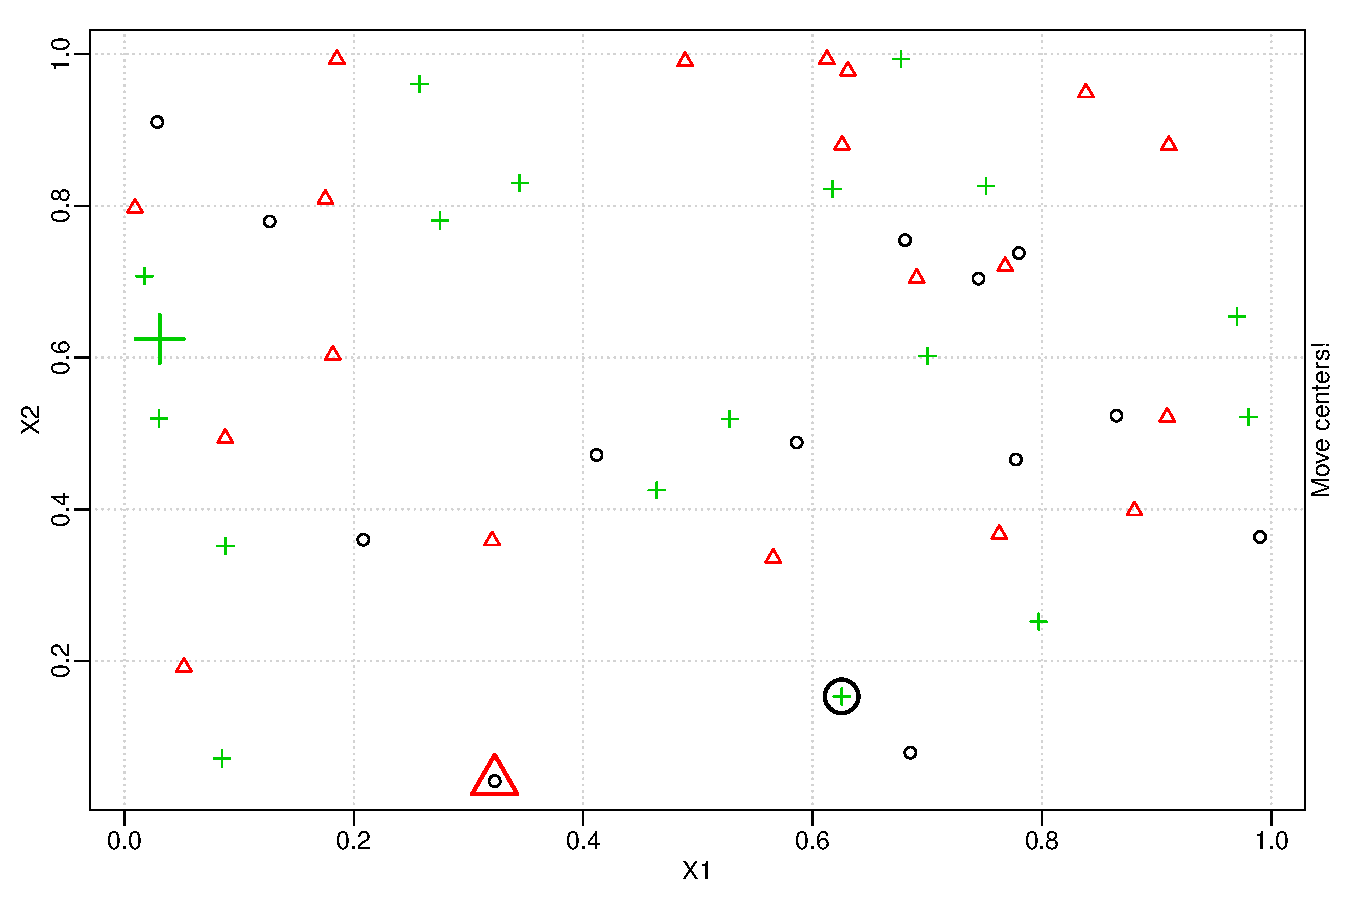
\includegraphics[width=.8\textwidth]{figures/unnamed-chunk-1-1} 

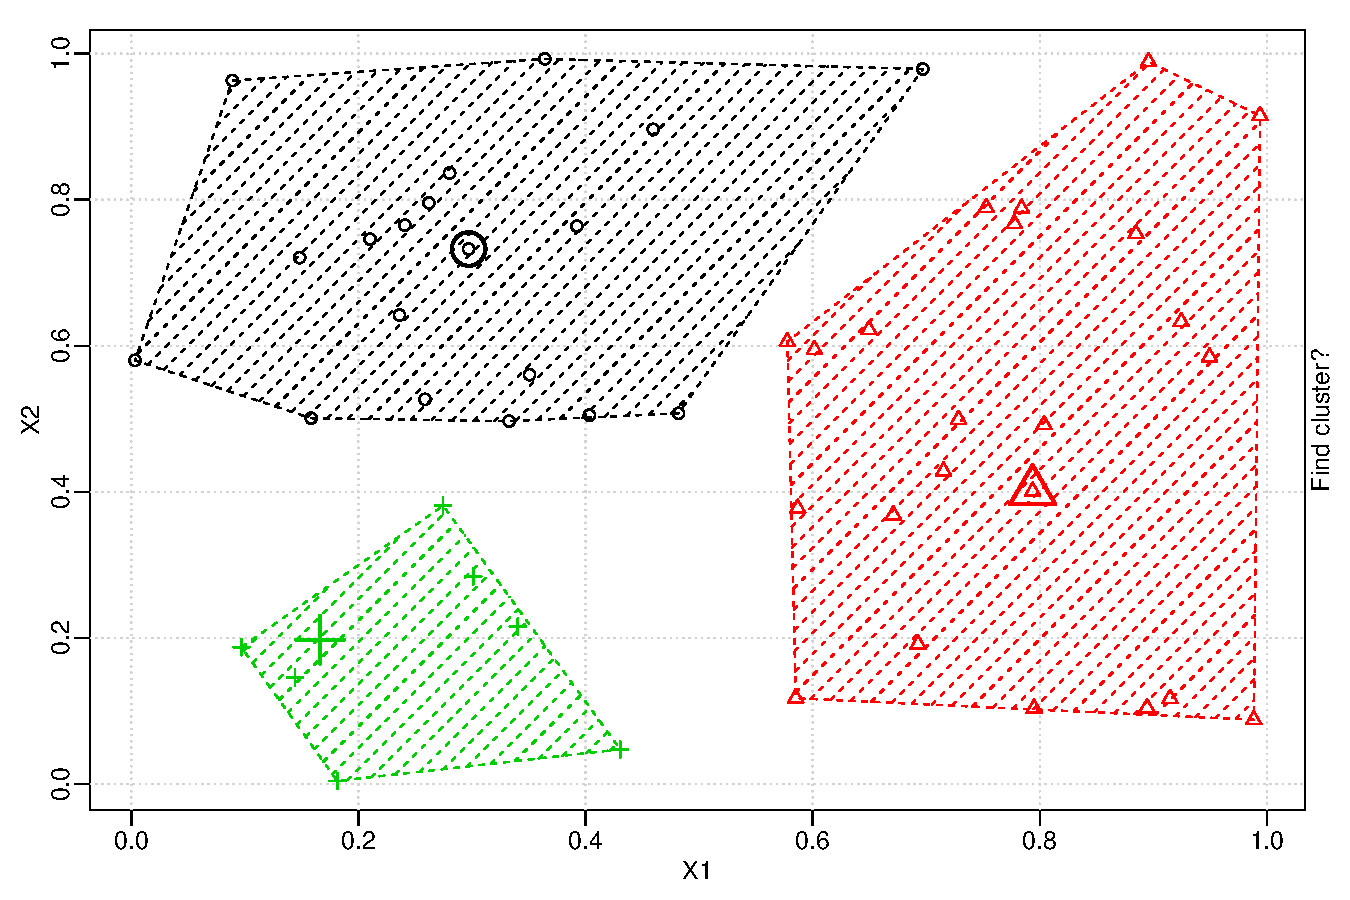
\includegraphics[width=.8\textwidth]{figures/unnamed-chunk-1-2} 

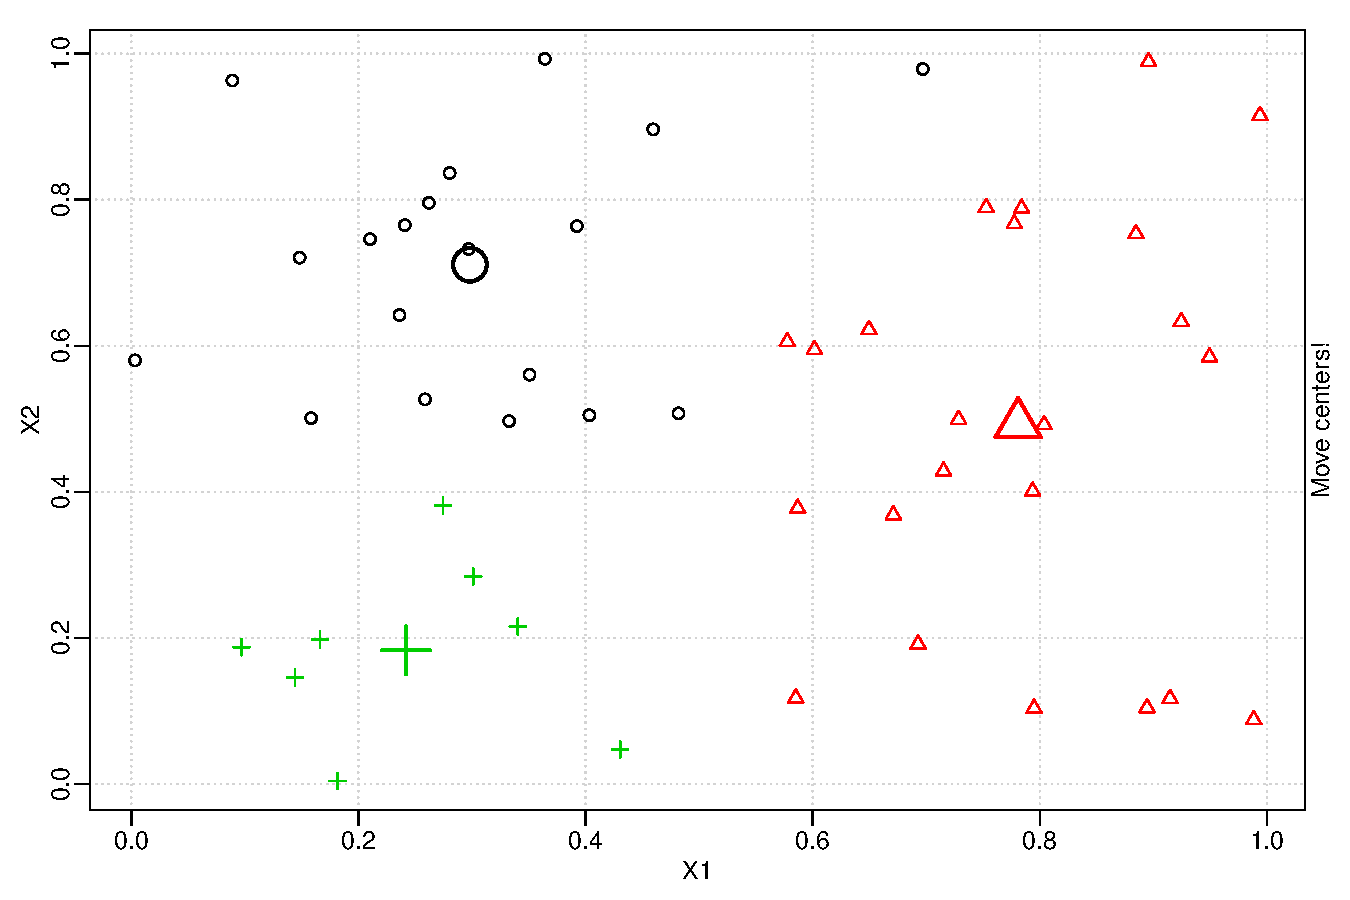
\includegraphics[width=.8\textwidth]{figures/unnamed-chunk-1-3} 

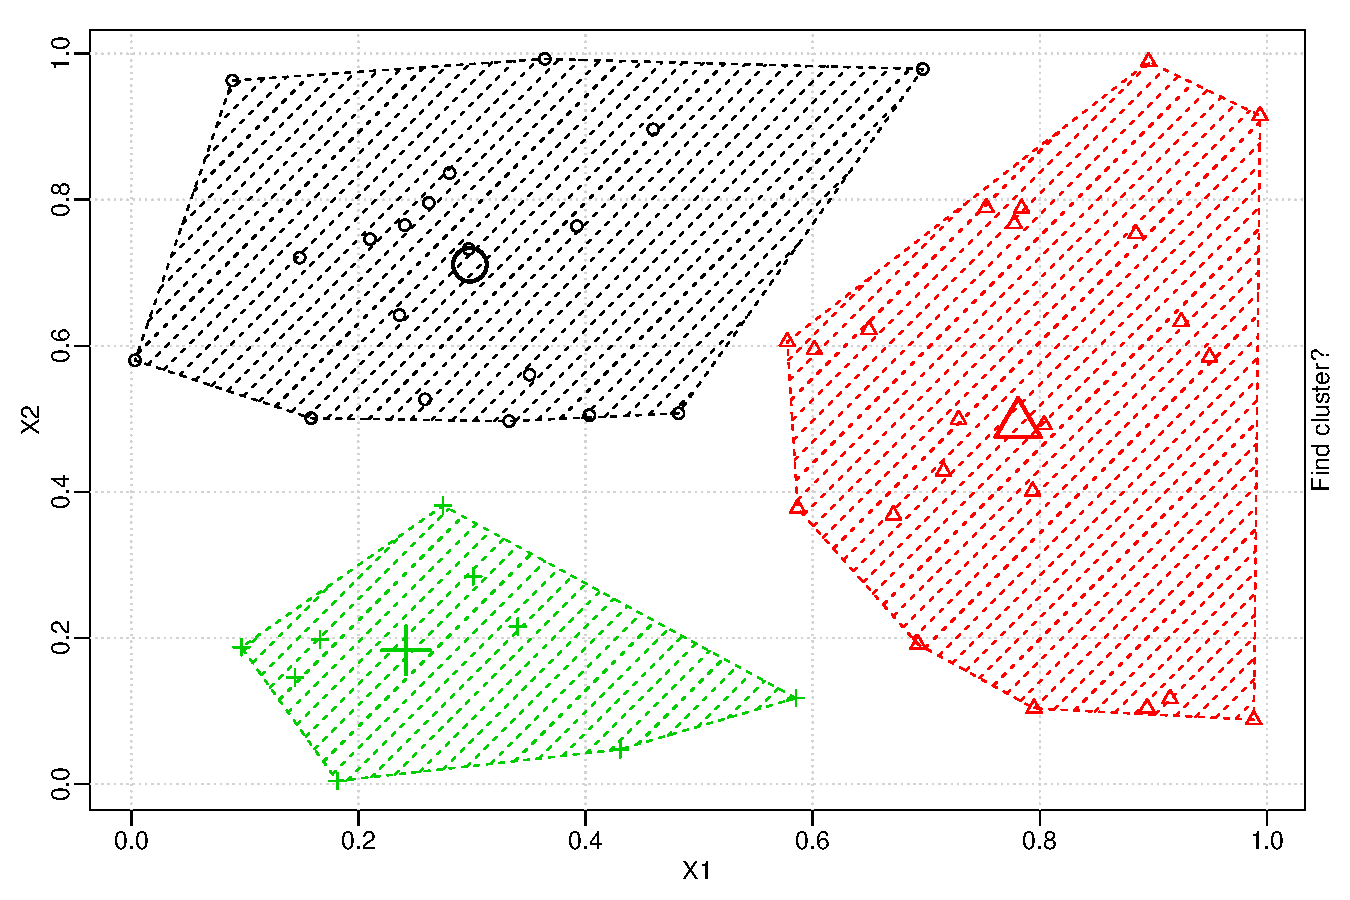
\includegraphics[width=.8\textwidth]{figures/unnamed-chunk-1-4} 

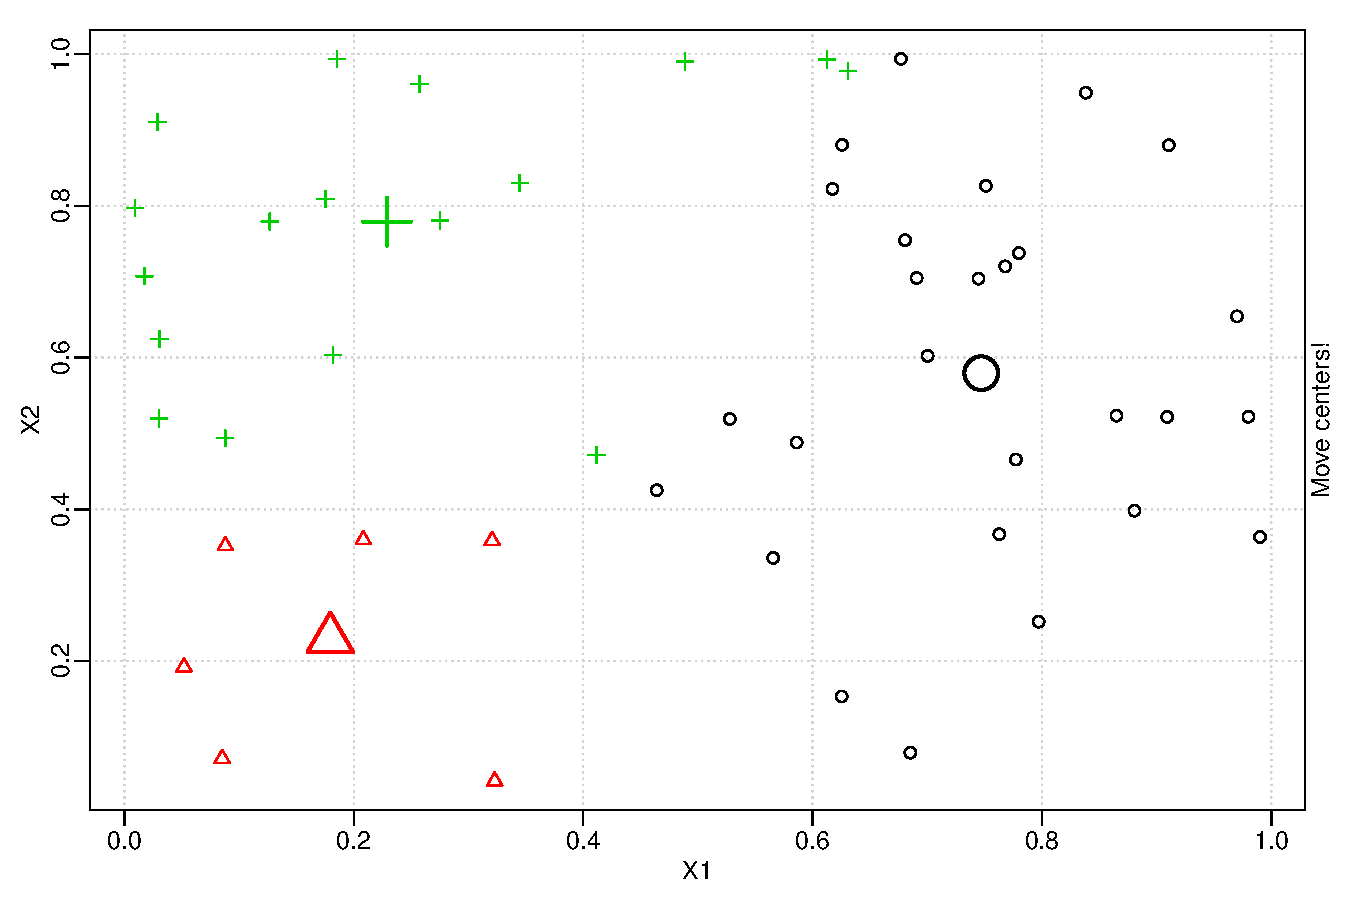
\includegraphics[width=.8\textwidth]{figures/unnamed-chunk-1-5} 

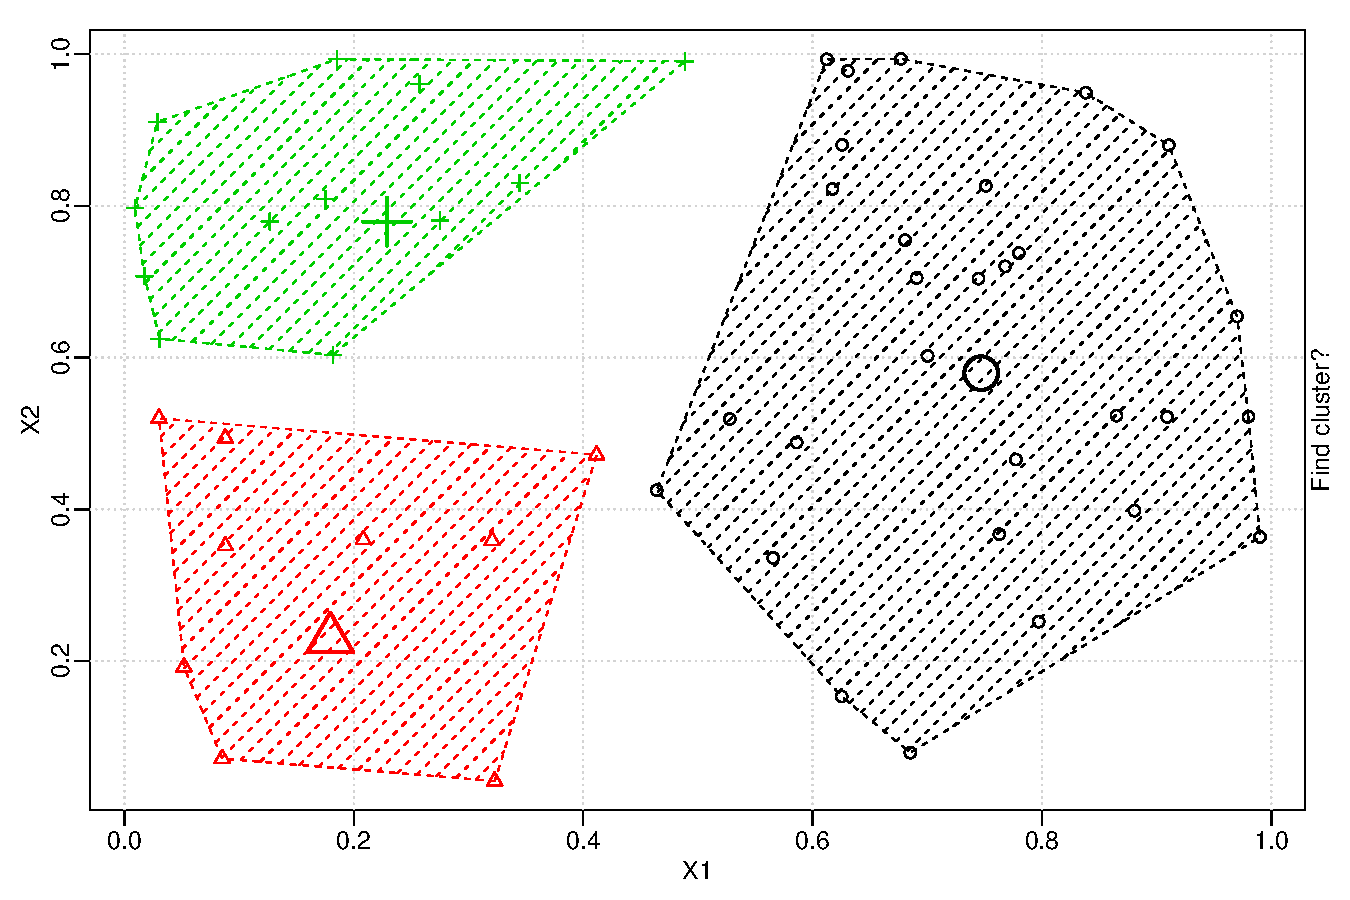
\includegraphics[width=.8\textwidth]{figures/unnamed-chunk-1-6} 

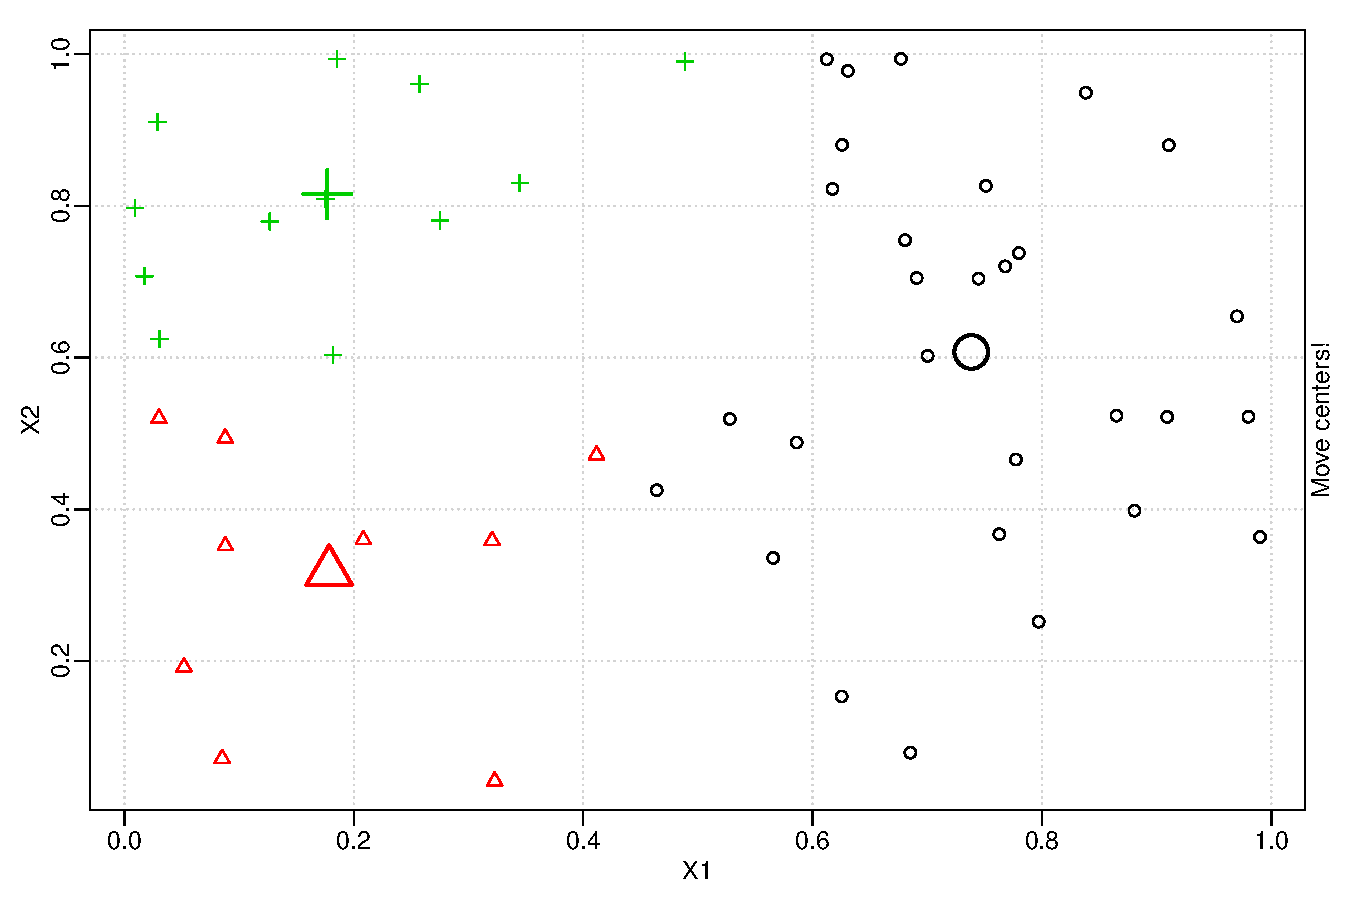
\includegraphics[width=.8\textwidth]{figures/unnamed-chunk-1-7} 

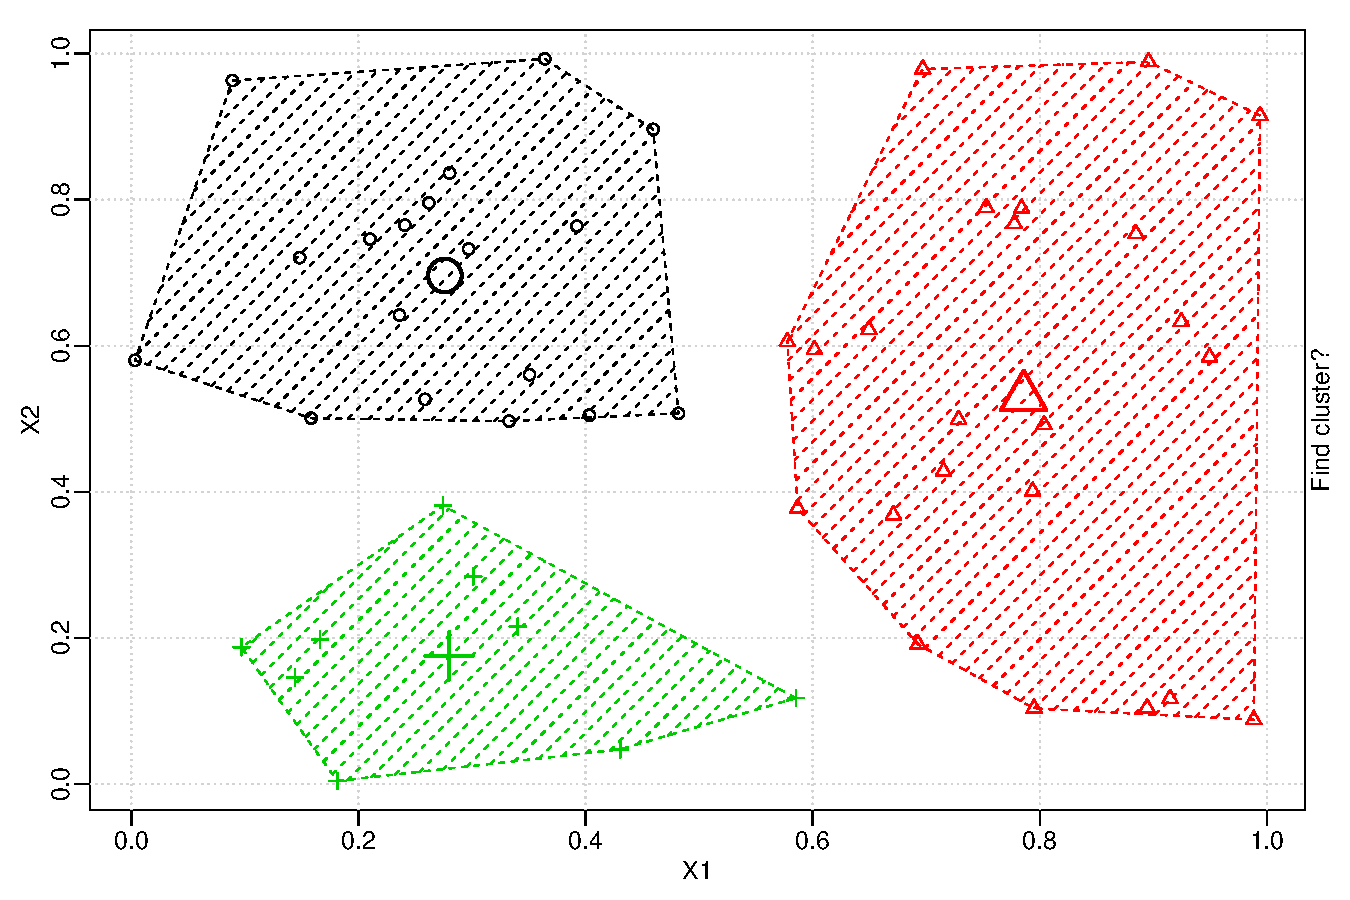
\includegraphics[width=.8\textwidth]{figures/unnamed-chunk-1-8} 

\end{knitrout}

\end{frame}

\begin{frame}
\frametitle{K-means: properties}
  
  \begin{block}{Other schemes}
    \begin{itemize}
      \item \alert{McQueen}: modify the mean each time a sample is assigned to a new cluster.
      \item \alert{Hartigan}: modify the mean by removing the considered sample, assign it to the nearby center and recompute the new mean after assignment.
    \end{itemize}
  \end{block}
  
  \begin{block}{Initialization}
    No guarantee to converge to a global optimum
    \begin{itemize}
      \item Repeat and keep the best result
      \item k-Mean++: try to take them as separated as possible.
    \end{itemize}
  \end{block}

  \begin{block}{Complexity}
     $O(n K T)$ where $T$ is the number of step in the algorithm.
  \end{block}
  
\end{frame}

\begin{frame}[fragile,allowframebreaks]
  \frametitle{K-means in \texttt{R} on uncorrected data set}

\begin{knitrout}\scriptsize
\definecolor{shadecolor}{rgb}{0.969, 0.969, 0.969}\color{fgcolor}\begin{kframe}
\begin{alltt}
\hlstd{uncor_kmeans_res} \hlkwb{<-} \hlstd{crabs} \hlopt
  \hlkwd{select}\hlstd{(}\hlopt{-}\hlstd{species,} \hlopt{-}\hlstd{sex)} \hlopt
  \hlkwd{kmeans}\hlstd{(}\hlnum{4}\hlstd{,} \hlkwc{nstart} \hlstd{=} \hlnum{10}\hlstd{)}
\hlstd{uncor_clusters} \hlkwb{<-} \hlkwd{as.factor}\hlstd{(uncor_kmeans_res}\hlopt{$}\hlstd{cluster)}
\hlstd{uncor_centers}  \hlkwb{<-} \hlkwd{as_tibble}\hlstd{(uncor_kmeans_res}\hlopt{$}\hlstd{centers)}
\hlstd{classes} \hlkwb{<-} \hlkwd{paste}\hlstd{(crabs_corrected}\hlopt{$}\hlstd{species, crabs_corrected}\hlopt{$}\hlstd{sex,} \hlkwc{sep} \hlstd{=} \hlstr{"-"}\hlstd{)}

\hlstd{crabs} \hlopt
  \hlkwd{ggplot}\hlstd{(}\hlkwd{aes}\hlstd{(}\hlkwc{x} \hlstd{= carapace_length,} \hlkwc{y} \hlstd{= carapace_width,} \hlkwc{color} \hlstd{= uncor_clusters))} \hlopt{+}
  \hlkwd{geom_point}\hlstd{(}\hlkwd{aes}\hlstd{(}\hlkwc{shape} \hlstd{= classes))} \hlopt{+}
  \hlkwd{geom_point}\hlstd{(}\hlkwc{data} \hlstd{= uncor_centers,} \hlkwc{color} \hlstd{=} \hlstr{'coral'}\hlstd{,} \hlkwc{size} \hlstd{=} \hlnum{4} \hlstd{,} \hlkwc{pch} \hlstd{=} \hlnum{21}\hlstd{)} \hlopt{+}
  \hlkwd{geom_point}\hlstd{(}\hlkwc{data} \hlstd{= uncor_centers,} \hlkwc{color} \hlstd{=} \hlstr{'coral'}\hlstd{,} \hlkwc{size} \hlstd{=} \hlnum{50}\hlstd{,} \hlkwc{alpha} \hlstd{=} \hlnum{0.2}\hlstd{)}
\end{alltt}
\end{kframe}
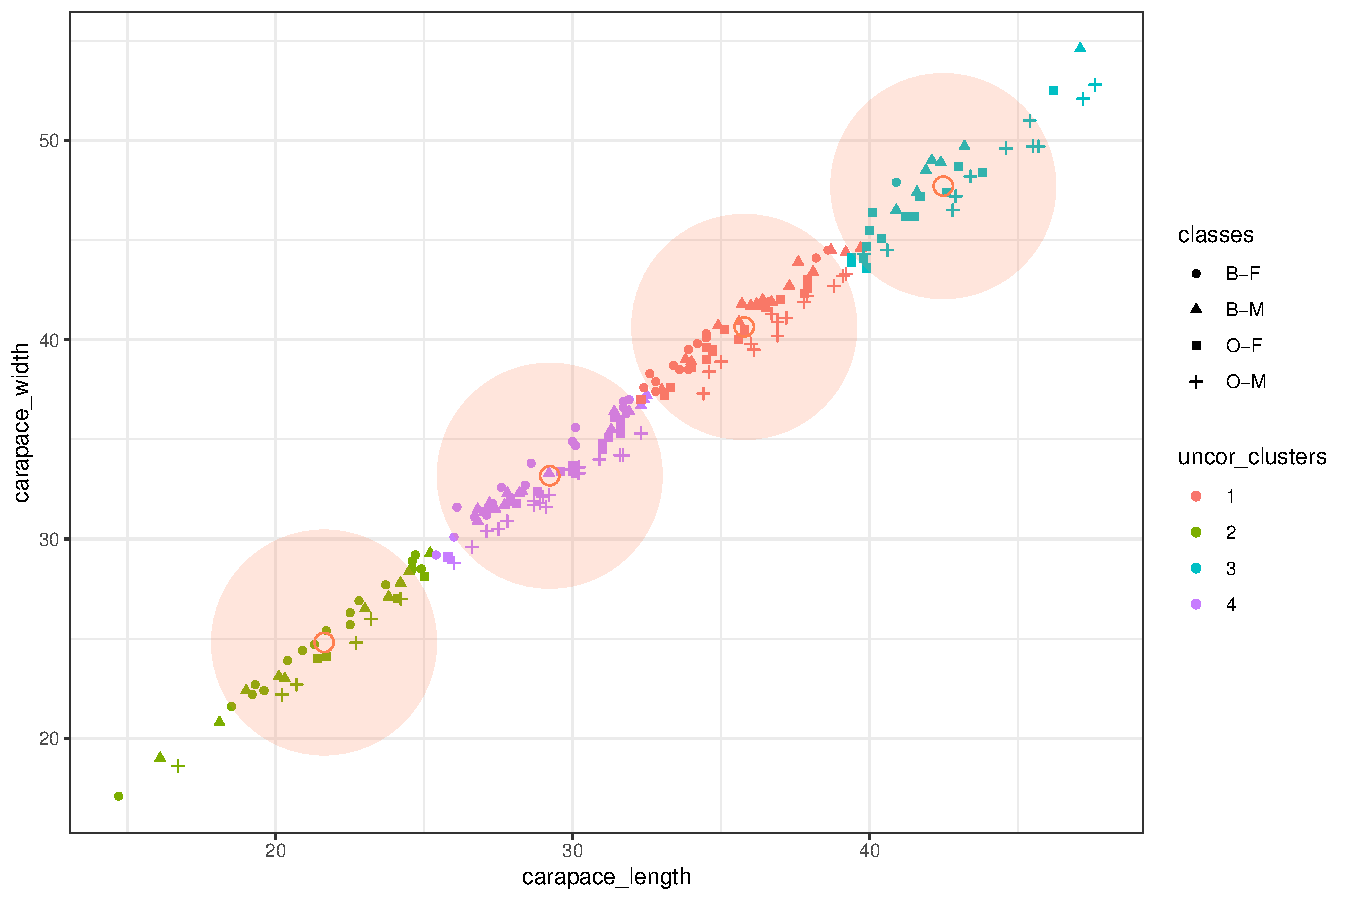
\includegraphics[width=.8\textwidth]{figures/kmeans_uncorrected_crabs-1} 

\end{knitrout}
  
\end{frame}

\begin{frame}[fragile,allowframebreaks]
  \frametitle{K-means in \texttt{R} on corrected crabs data set}
  
\begin{knitrout}\scriptsize
\definecolor{shadecolor}{rgb}{0.969, 0.969, 0.969}\color{fgcolor}\begin{kframe}
\begin{alltt}
\hlstd{kmeans_res} \hlkwb{<-} \hlstd{crabs_corrected} \hlopt
  \hlkwd{select}\hlstd{(}\hlopt{-}\hlstd{species,} \hlopt{-}\hlstd{sex)} \hlopt
  \hlkwd{kmeans}\hlstd{(}\hlnum{4}\hlstd{,} \hlkwc{nstart} \hlstd{=} \hlnum{10}\hlstd{)}
\hlstd{clusters} \hlkwb{<-} \hlkwd{as.factor}\hlstd{(kmeans_res}\hlopt{$}\hlstd{cluster)}
\hlstd{centers}  \hlkwb{<-} \hlkwd{as.tibble}\hlstd{(kmeans_res}\hlopt{$}\hlstd{centers)}
\hlstd{classes} \hlkwb{<-} \hlkwd{paste}\hlstd{(crabs_corrected}\hlopt{$}\hlstd{species, crabs_corrected}\hlopt{$}\hlstd{sex,} \hlkwc{sep} \hlstd{=} \hlstr{"-"}\hlstd{)}

\hlstd{crabs_corrected} \hlopt
  \hlkwd{ggplot}\hlstd{(}\hlkwd{aes}\hlstd{(}\hlkwc{x} \hlstd{= carapace_length,} \hlkwc{y} \hlstd{= carapace_width,} \hlkwc{color} \hlstd{= clusters))} \hlopt{+}
  \hlkwd{geom_point}\hlstd{(}\hlkwd{aes}\hlstd{(}\hlkwc{shape} \hlstd{= classes))} \hlopt{+}
  \hlkwd{geom_point}\hlstd{(}\hlkwc{data} \hlstd{= centers,} \hlkwc{color} \hlstd{=} \hlstr{'coral'}\hlstd{,} \hlkwc{size} \hlstd{=} \hlnum{4} \hlstd{,} \hlkwc{pch} \hlstd{=} \hlnum{21}\hlstd{)} \hlopt{+}
  \hlkwd{geom_point}\hlstd{(}\hlkwc{data} \hlstd{= centers,} \hlkwc{color} \hlstd{=} \hlstr{'coral'}\hlstd{,} \hlkwc{size} \hlstd{=} \hlnum{50}\hlstd{,} \hlkwc{alpha} \hlstd{=} \hlnum{0.2}\hlstd{)}
\end{alltt}
\end{kframe}
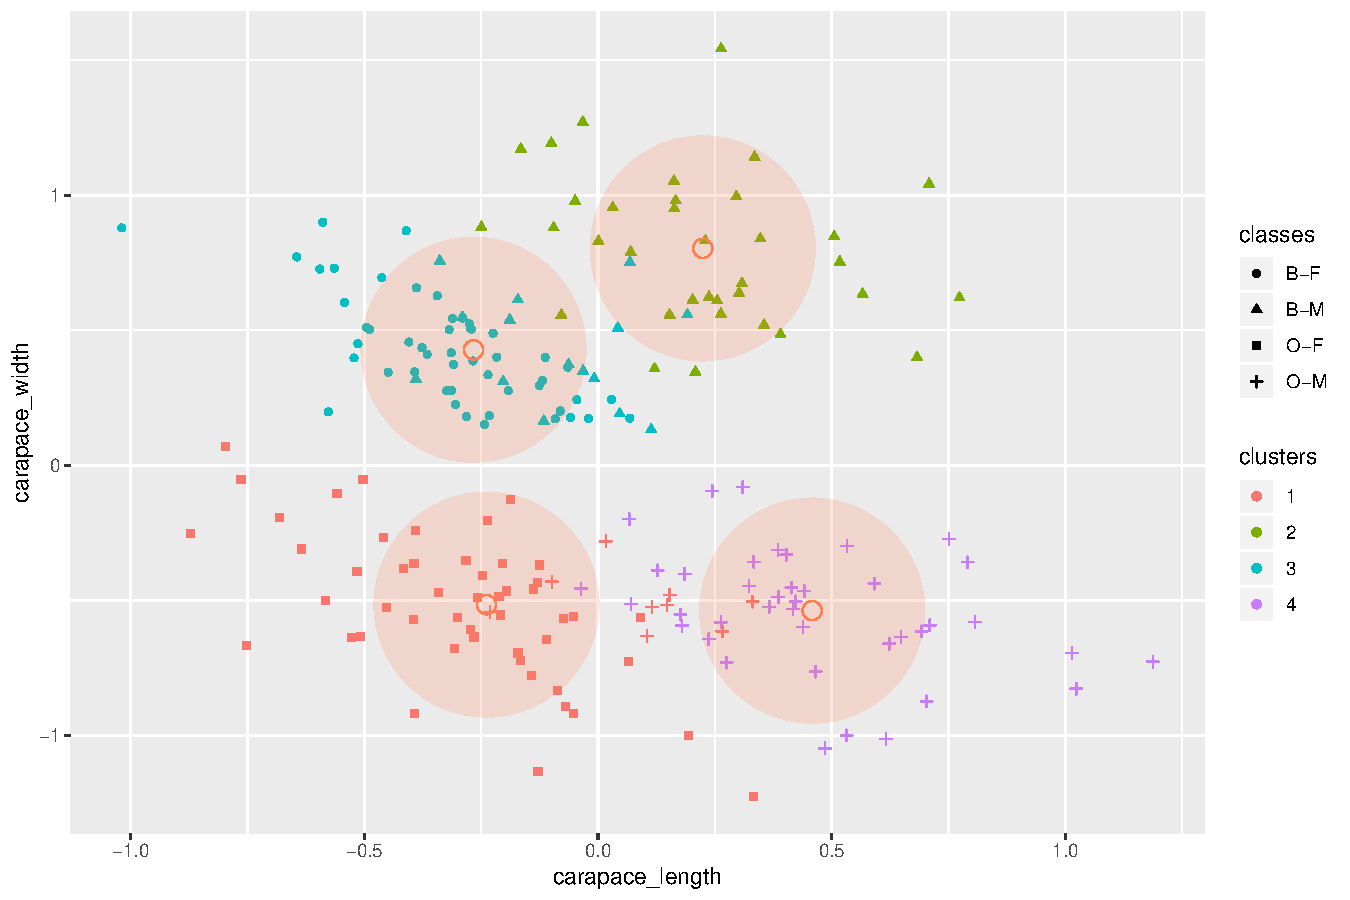
\includegraphics[width=.8\textwidth]{figures/kmeans_crabs-1} 

\end{knitrout}

\end{frame}

% <<spectral kmeans crabs>>=
% SVD <- svd(select(crabs_corrected, -species, -sex))
% spec_crabs <- as.tibble(SVD$u[,1:2] %*% diag(SVD$d[1:2]))
% spec_kmeans_res <- spec_crabs %>%
%   kmeans(4, nstart = 10)
% spec_clusters <- as.factor(spec_kmeans_res$cluster)
% spec_centers  <- as.tibble(spec_kmeans_res$centers)
% classes <- paste(crabs_corrected$species, crabs_corrected$sex, sep = "-")
% 
% ggplot(spec_crabs, aes(V1, V2, color = spec_clusters)) +
%   geom_point(aes(shape = classes)) +
%   geom_point(data = spec_centers, color = 'coral', size = 4 , pch = 21) +
%   geom_point(data = spec_centers, color = 'coral', size = 50, alpha = 0.2)
% @

\begin{frame}[fragile]
  \frametitle{Clustering comparison}

\begin{knitrout}\scriptsize
\definecolor{shadecolor}{rgb}{0.969, 0.969, 0.969}\color{fgcolor}\begin{kframe}
\begin{alltt}
\hlstd{aricode}\hlopt{::}\hlkwd{ARI}\hlstd{(clusters, classes)}
\end{alltt}
\begin{verbatim}
## [1] 0.7223637
\end{verbatim}
\begin{alltt}
\hlstd{aricode}\hlopt{::}\hlkwd{ARI}\hlstd{(uncor_clusters, classes)}
\end{alltt}
\begin{verbatim}
## [1] 0.01573617
\end{verbatim}
\end{kframe}
\end{knitrout}

\begin{knitrout}\scriptsize
\definecolor{shadecolor}{rgb}{0.969, 0.969, 0.969}\color{fgcolor}\begin{kframe}
\begin{alltt}
\hlstd{knitr}\hlopt{::}\hlkwd{kable}\hlstd{(}\hlkwd{table}\hlstd{(clusters, classes),}
\hlkwc{caption} \hlstd{=} \hlstr{"Estimating structure with k-means"}\hlstd{)}
\end{alltt}
\end{kframe}\begin{table}

\caption{\label{tab:contingency_table_kmeans}Estimating structure with k-means}
\centering
\begin{tabular}[t]{r|r|r|r}
\hline
B-F & B-M & O-F & O-M\\
\hline
0 & 35 & 0 & 0\\
\hline
0 & 0 & 50 & 9\\
\hline
0 & 0 & 0 & 41\\
\hline
50 & 15 & 0 & 0\\
\hline
\end{tabular}
\end{table}


\end{knitrout}

\end{frame}

\subsection{Hierarchical Agglomerative Clustering}

\begin{frame}
  \frametitle{Agglomerative Clustering: Heuristic}
    
    \begin{block}{Idea}
      \begin{enumerate}
        \item Start with small clusters (\textit{e.g.} one cluster $\equiv$ one individual)
        \item Merge the most similar clusters sequentially (and greedily)
        \item Stops when all individuals are in the same groups
      \end{enumerate}
    \end{block}

    \begin{block}{Ingredients}
      \begin{enumerate}
        \item a dissimilarity measure (distance between individuals)
        \item a merging criterion $\Delta$ (dissimilarity between clusters)
      \end{enumerate}
    \end{block}

    \begin{itemize}
      \item[+] Generates a hierarchy of clustering instead of a single partition
      \item[--] Need to select the number of cluster afterwards
    \end{itemize}
\end{frame}

\begin{frame}
  \frametitle{Agglomerative Clustering: general algorithm}

  \begin{block}{Algorithm}
    \vspace{-.25cm}
    \begin{enumerate}
      \item Start with $(\mathcal{C}_k^{(0)})= (\{ \bx_i \})$ the collection of all singletons.
      \item At step $s$, we have $n-s$ clusters $(\mathcal{C}_{k}^{(s)})$:

      \begin{itemize}
        \item Find the two most similar clusters according to a criterion $\Delta$:%%\\[-.75cm]
        \begin{align*}
          (k,\ell) = \argmin_{(k',\ell')} \Delta(\mathcal{C}_{k'}^{(s)},\mathcal{C}_{_ell'}^{(s)})
        \end{align*}
        \item Merge $\mathcal{C}_{k}^{(s)}$ and $\mathcal{C}_{\ell}^{(s)}$ into $\mathcal{C}_{k}^{(s+1)}$
        \item Update the distances between $\mathcal{C}_{k}^{(s+1)}$ and the remaining clusters
      \end{itemize}
  
      \item Repeat until there is only one cluster.
    \end{enumerate}
  \end{block}

  \vfill

  \begin{block}{Complexity}<2>
    \vspace{-.25cm}
    \begin{itemize}
      \item In general $O(n^3)$
      \item Can be reduced to $O(n^2)$ if boundering the number of merges
    \end{itemize}
  \end{block}
  
\end{frame}

\begin{frame}

  \begin{center}
    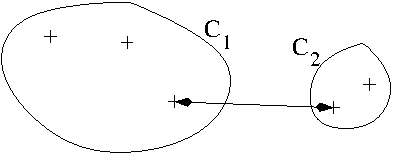
\includegraphics[width=.3\textwidth]{ex_sautmin}
    \hspace*{.1\textwidth}
    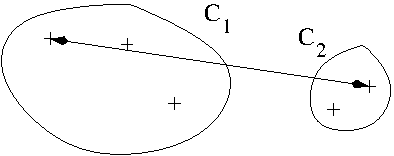
\includegraphics[width=.3\textwidth]{ex_sautmax}
  \end{center}

  \begin{block}{Merging criterion based on the distance between points}
    \begin{itemize}
      \item Single linkage (or minimum linkage):
      \begin{align*}
        \Delta(\mathcal{C}_k, \mathcal{C}_\ell) = \min_{\bx_i \in \mathcal{C}_k, \bx_j \in \mathcal{C}_\ell} d(\bx_i, \bx_j)
      \end{align*}
      \item Complete linkage (or maximum linkage):
      \begin{align*}
        \Delta(\mathcal{C}_k, \mathcal{C}_\ell) = \max_{\bx_i \in \mathcal{C}_k} \max_{\bx_j \in \mathcal{C}_\ell}d(\bx_i, \bx_j)
    \end{align*}
    \item Average linkage (or group linkage):
      \begin{align*}
        \Delta(\mathcal{C}_k, \mathcal{C}_\ell) = \frac{1}{|\mathcal{C}_k||\mathcal{C}_\ell|} \sum_{\bx_i \in \mathcal{C}_k}\sum_{\bx_ \in\mathcal{C}_\ell} d(\bx_i, \bx_j)
      \end{align*}
    \end{itemize}
  \end{block}

\end{frame}

\begin{frame}
  \frametitle{Ward's criteria}
  
  \begin{block}{Merging criterion based on distance to the mean}
    Ward's criterion:
    \begin{align*}
      \Delta(\mathcal{C}_k, \mathcal{C}_\ell) 
        & = \sum_{\bx_i \in \mathcal{C}_k} \left( d^2(\bx_i, \bmu_{\mathcal{C}_k \cup \mathcal{C}_\ell} ) - d^2(\bx_i, \bmu_{\mathcal{C}_k}) \right) \\
        & \quad + \sum_{\bx_j \in \mathcal{C}_\ell} \left( d^2(\bx_j, \bmu_{\mathcal{C}_j \cup \mathcal{C}_\ell} ) - d^2(\bx_j, \bmu_{\mathcal{C}_\ell}) \right)
      \end{align*}
    \end{block}

    \begin{block}{Euclidean case}
       If $d$ is the Euclidean distance, then
      \begin{align*}
        \Delta(\mathcal{C}_k, \mathcal{C}_\ell) = \frac{2|\mathcal{C}_k||\mathcal{C}_\ell|}{|\mathcal{C}_k|+|\mathcal{C}_\ell|}d^2(\bmu_{\mathcal{C}_k}, \bmu_{\mathcal{C}_\ell})
      \end{align*}
    \end{block}

\end{frame}

\begin{frame}
  \frametitle{Ward's criteria: details}
  
  Recall that the inertia measures the homogenity of th size-K clustering
  \begin{equation*}
    I_W = \sum_{k=1}^K \sum_{\bx_i \in \mathcal{C}_k} \| \bx_i - \bmu_{\mathcal{C}_k}  \|_2^2, \quad I_B = \sum_{k=1}^K n_k \| \bmu_k - \bmu  \|_2^2
  \end{equation*}
  
  \onslide<2->{
  Consider the following two partitions 
  \begin{itemize}
    \item  $\mathcal{P} = (\mathcal{C}_1, \dots,\mathcal{C}_K)$ at one level of the hierarchy $\Omega$
    \item  $\mathcal{P}'$ is $\mathcal{P}$ once $\mathcal{C}_k, \mathcal{C}_\ell$ merged
  \end{itemize}
  Then
  \begin{equation*}
    I_B(\mathcal{P}) - I_B(\mathcal{P'}) = \frac{|\mathcal{C}_k||\mathcal{C}_\ell|}{|\mathcal{C}_k|+|\mathcal{C}_\ell|}d^2(\bmu_{\mathcal{C}_k}, \bmu_{\mathcal{C}_\ell}) = \frac{1}{2} \Delta(\mathcal{C}_k, \mathcal{C}_\ell).
  \end{equation*}
  }

  \onslide<3>{
  \begin{itemize}
    \item[$\rightsquigarrow$] At each step, Ward limits the loss (increase) of the intra (inter) class variance
    \item[$\rightsquigarrow$] Defines an indexed hierarchy (height of the dendrogram)
    \item[$\rightsquigarrow$] Same criteria as in the K-means algorithm
  \end{itemize}
  }

\end{frame}

\begin{frame}[fragile]
  \frametitle{Ward agglomerative clustering in \texttt{R}}
  
\begin{knitrout}\scriptsize
\definecolor{shadecolor}{rgb}{0.969, 0.969, 0.969}\color{fgcolor}\begin{kframe}
\begin{alltt}
\hlstd{Ward} \hlkwb{<-} \hlstd{crabs_corrected} \hlopt
  \hlkwd{select}\hlstd{(}\hlopt{-}\hlstd{sex,} \hlopt{-}\hlstd{species)} \hlopt
  \hlkwd{dist}\hlstd{(}\hlkwc{method} \hlstd{=} \hlstr{"euclidean"}\hlstd{)} \hlopt
  \hlkwd{hclust}\hlstd{(}\hlkwc{method} \hlstd{=} \hlstr{"ward.D2"}\hlstd{)}
\hlkwd{plot}\hlstd{(Ward)}
\end{alltt}
\end{kframe}
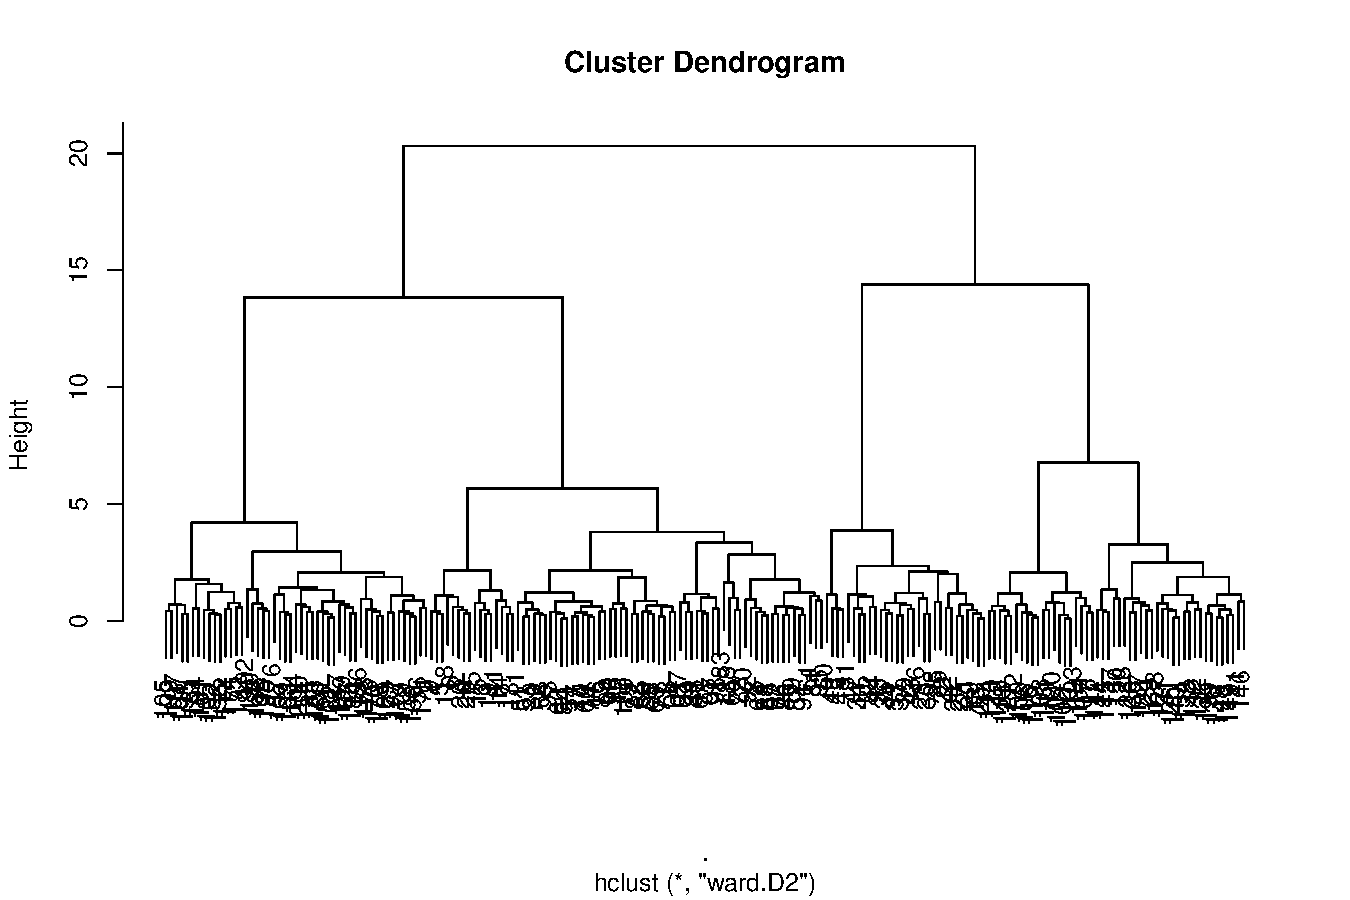
\includegraphics[width=.8\textwidth]{figures/Ward-1} 

\end{knitrout}

\end{frame}

\begin{frame}[fragile,allowframebreaks]
  \frametitle{Ward agglomerative clustering in \texttt{R}: comparison}

Compare with out reference classification and k-means
\begin{knitrout}\scriptsize
\definecolor{shadecolor}{rgb}{0.969, 0.969, 0.969}\color{fgcolor}\begin{kframe}
\begin{alltt}
\hlstd{aricode}\hlopt{::}\hlkwd{ARI}\hlstd{(}\hlkwd{cutree}\hlstd{(Ward,} \hlnum{4}\hlstd{), classes)}
\end{alltt}
\begin{verbatim}
## [1] 0.6829729
\end{verbatim}
\begin{alltt}
\hlstd{aricode}\hlopt{::}\hlkwd{ARI}\hlstd{(}\hlkwd{cutree}\hlstd{(Ward,} \hlnum{4}\hlstd{), clusters)}
\end{alltt}
\begin{verbatim}
## [1] 0.7999974
\end{verbatim}
\end{kframe}
\end{knitrout}

\begin{knitrout}\scriptsize
\definecolor{shadecolor}{rgb}{0.969, 0.969, 0.969}\color{fgcolor}\begin{kframe}
\begin{alltt}
\hlstd{knitr}\hlopt{::}\hlkwd{kable}\hlstd{(}\hlkwd{table}\hlstd{(clusters,} \hlkwd{cutree}\hlstd{(Ward,}\hlnum{4}\hlstd{)),}
\hlkwc{caption} \hlstd{=} \hlstr{"k-means vs Ward"}\hlstd{)}
\end{alltt}
\end{kframe}\begin{table}

\caption{\label{tab:contingency_table_kmeans_vs_ward}k-means vs Ward}
\centering
\begin{tabular}[t]{r|r|r|r}
\hline
1 & 2 & 3 & 4\\
\hline
5 & 30 & 0 & 0\\
\hline
2 & 0 & 49 & 8\\
\hline
1 & 0 & 0 & 40\\
\hline
65 & 0 & 0 & 0\\
\hline
\end{tabular}
\end{table}


\end{knitrout}


Optimize over a range of values
\begin{knitrout}\scriptsize
\definecolor{shadecolor}{rgb}{0.969, 0.969, 0.969}\color{fgcolor}\begin{kframe}
\begin{alltt}
\hlstd{Ward} \hlopt  \hlkwd{cutree}\hlstd{(}\hlkwc{k} \hlstd{=} \hlnum{1}\hlopt{:}\hlnum{10}\hlstd{)} \hlopt  \hlkwd{as.data.frame}\hlstd{()} \hlopt \hlkwd{as.list}\hlstd{()} \hlopt
  \hlkwd{sapply}\hlstd{(aricode}\hlopt{::}\hlstd{ARI, classes)} \hlopt \hlkwd{plot}\hlstd{(}\hlkwc{type} \hlstd{=} \hlstr{"l"}\hlstd{)}
\end{alltt}
\end{kframe}
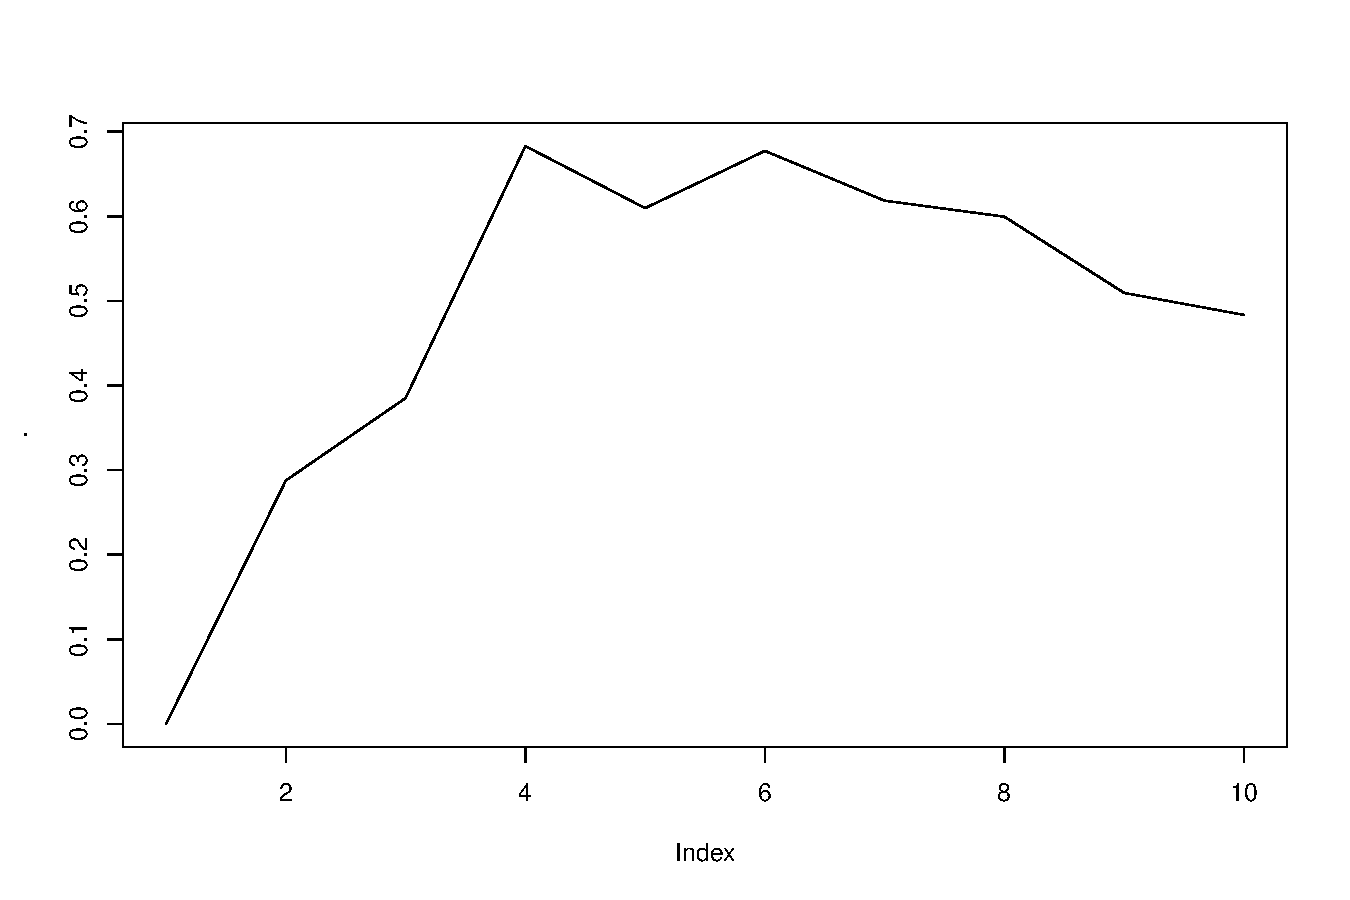
\includegraphics[width=.8\textwidth]{figures/Ward_ARIs-1} 

\end{knitrout}

Look at Ward intra-class variance
\begin{knitrout}\scriptsize
\definecolor{shadecolor}{rgb}{0.969, 0.969, 0.969}\color{fgcolor}\begin{kframe}
\begin{alltt}
\hlkwd{plot}\hlstd{(}\hlkwd{rev}\hlstd{(Ward}\hlopt{$}\hlstd{height)[}\hlnum{1}\hlopt{:}\hlnum{20}\hlstd{],} \hlkwc{xlab} \hlstd{=} \hlstr{"number of clusters"}\hlstd{,} \hlkwc{ylab} \hlstd{=} \hlstr{"height"}\hlstd{)}
\end{alltt}
\end{kframe}
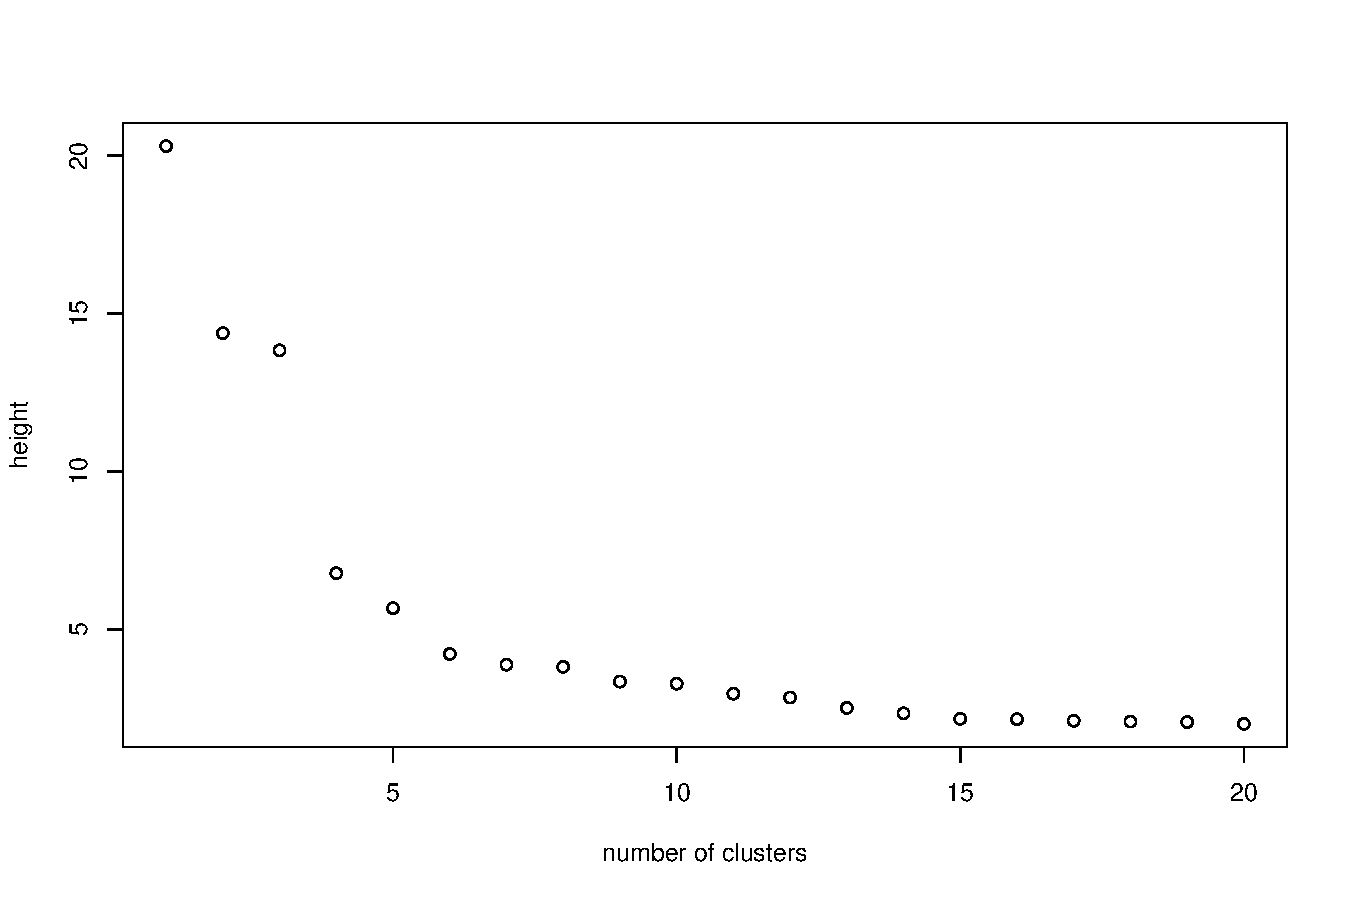
\includegraphics[width=.8\textwidth]{figures/criteria-1} 

\end{knitrout}

\end{frame}

\begin{frame}[fragile,allowframebreaks]
  \frametitle{Ward agglomerative clustering in \texttt{R}: projection}

\begin{knitrout}\scriptsize
\definecolor{shadecolor}{rgb}{0.969, 0.969, 0.969}\color{fgcolor}\begin{kframe}
\begin{alltt}
\hlstd{clusters_ward} \hlkwb{<-} \hlkwd{as.factor}\hlstd{(}\hlkwd{cutree}\hlstd{(Ward,} \hlnum{4}\hlstd{))}
\hlstd{centers_ward}  \hlkwb{<-} \hlkwd{select}\hlstd{(crabs_corrected,} \hlopt{-}\hlstd{sex,} \hlopt{-}\hlstd{species)} \hlopt
  \hlkwd{aggregate}\hlstd{(}\hlkwd{list}\hlstd{(}\hlkwd{cutree}\hlstd{(Ward,} \hlnum{4}\hlstd{)), mean)} \hlopt \hlkwd{as_tibble}\hlstd{()} \hlopt \hlkwd{select}\hlstd{(}\hlopt{-}\hlstd{Group.1)}

\hlstd{crabs_corrected} \hlopt
  \hlkwd{ggplot}\hlstd{(}\hlkwd{aes}\hlstd{(}\hlkwc{x} \hlstd{= carapace_length,} \hlkwc{y} \hlstd{= carapace_width,} \hlkwc{color} \hlstd{= clusters_ward))} \hlopt{+}
  \hlkwd{geom_point}\hlstd{(}\hlkwd{aes}\hlstd{(}\hlkwc{shape} \hlstd{= classes))} \hlopt{+}
  \hlkwd{geom_point}\hlstd{(}\hlkwc{data} \hlstd{= centers_ward,} \hlkwc{color} \hlstd{=} \hlstr{'coral'}\hlstd{,} \hlkwc{size} \hlstd{=} \hlnum{4} \hlstd{,} \hlkwc{pch} \hlstd{=} \hlnum{21}\hlstd{)} \hlopt{+}
  \hlkwd{geom_point}\hlstd{(}\hlkwc{data} \hlstd{= centers_ward,} \hlkwc{color} \hlstd{=} \hlstr{'coral'}\hlstd{,} \hlkwc{size} \hlstd{=} \hlnum{50}\hlstd{,} \hlkwc{alpha} \hlstd{=} \hlnum{0.2}\hlstd{)}
\end{alltt}
\end{kframe}
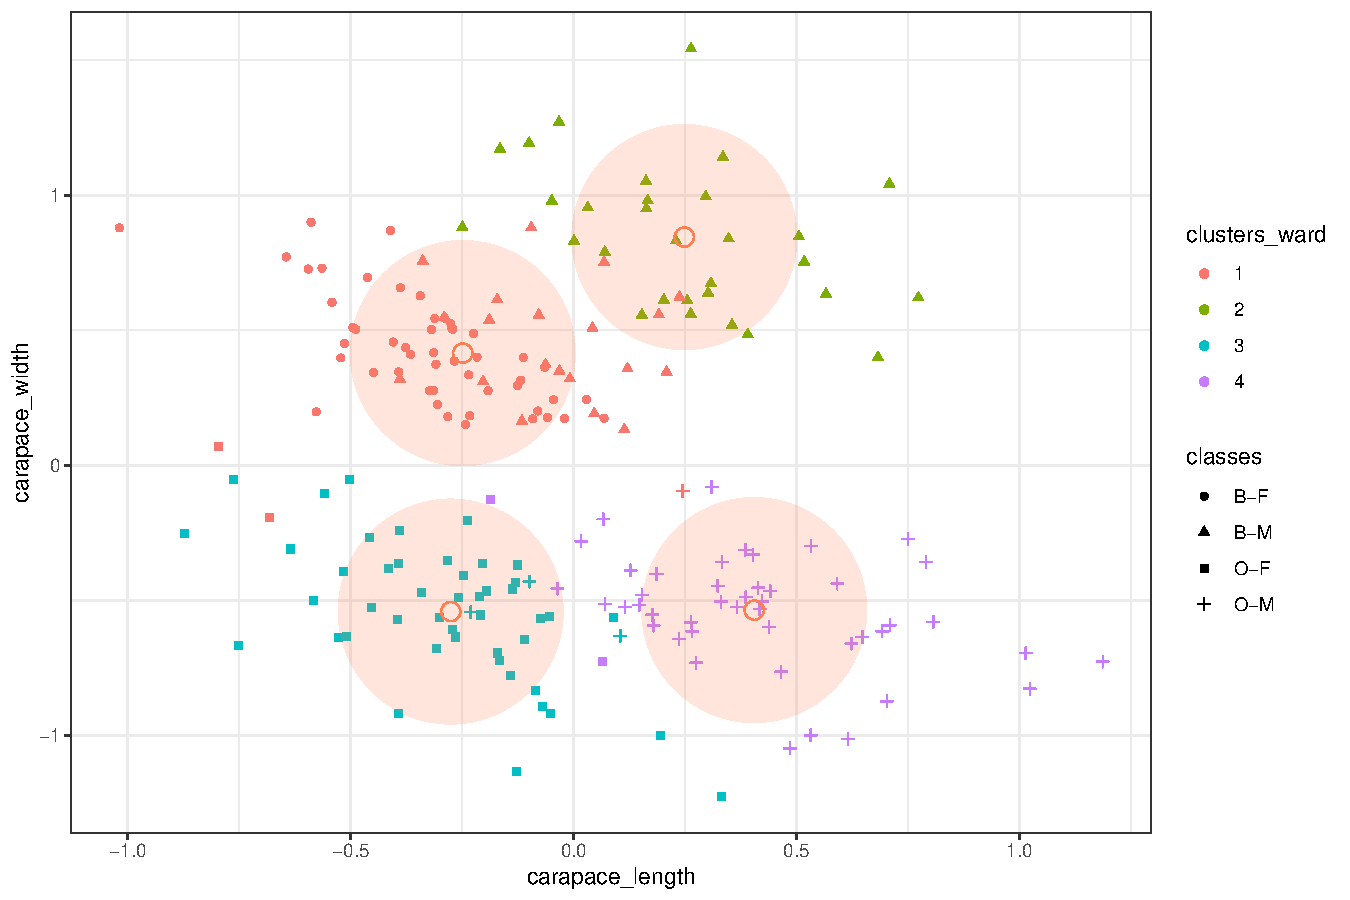
\includegraphics[width=.8\textwidth]{figures/Ward_projection-1} 

\end{knitrout}
\end{frame}

\begin{frame}[fragile]
  \frametitle{Reordered correlation matrix between individuals}
  
\begin{knitrout}\scriptsize
\definecolor{shadecolor}{rgb}{0.969, 0.969, 0.969}\color{fgcolor}\begin{kframe}
\begin{alltt}
\hlstd{C} \hlkwb{<-} \hlkwd{cor}\hlstd{(}\hlkwd{t}\hlstd{(}\hlkwd{select}\hlstd{(crabs_corrected,} \hlopt{-}\hlstd{sex,} \hlopt{-}\hlstd{species)))}
\hlstd{C} \hlkwb{<-} \hlstd{C[}\hlkwd{order}\hlstd{(clusters_ward),}\hlkwd{order}\hlstd{(clusters_ward)]}
  \hlkwd{corrplot}\hlstd{(C,} \hlkwc{method} \hlstd{=} \hlstr{"color"}\hlstd{,} \hlkwc{tl.pos} \hlstd{=} \hlstr{"n"}\hlstd{)}
\end{alltt}
\end{kframe}
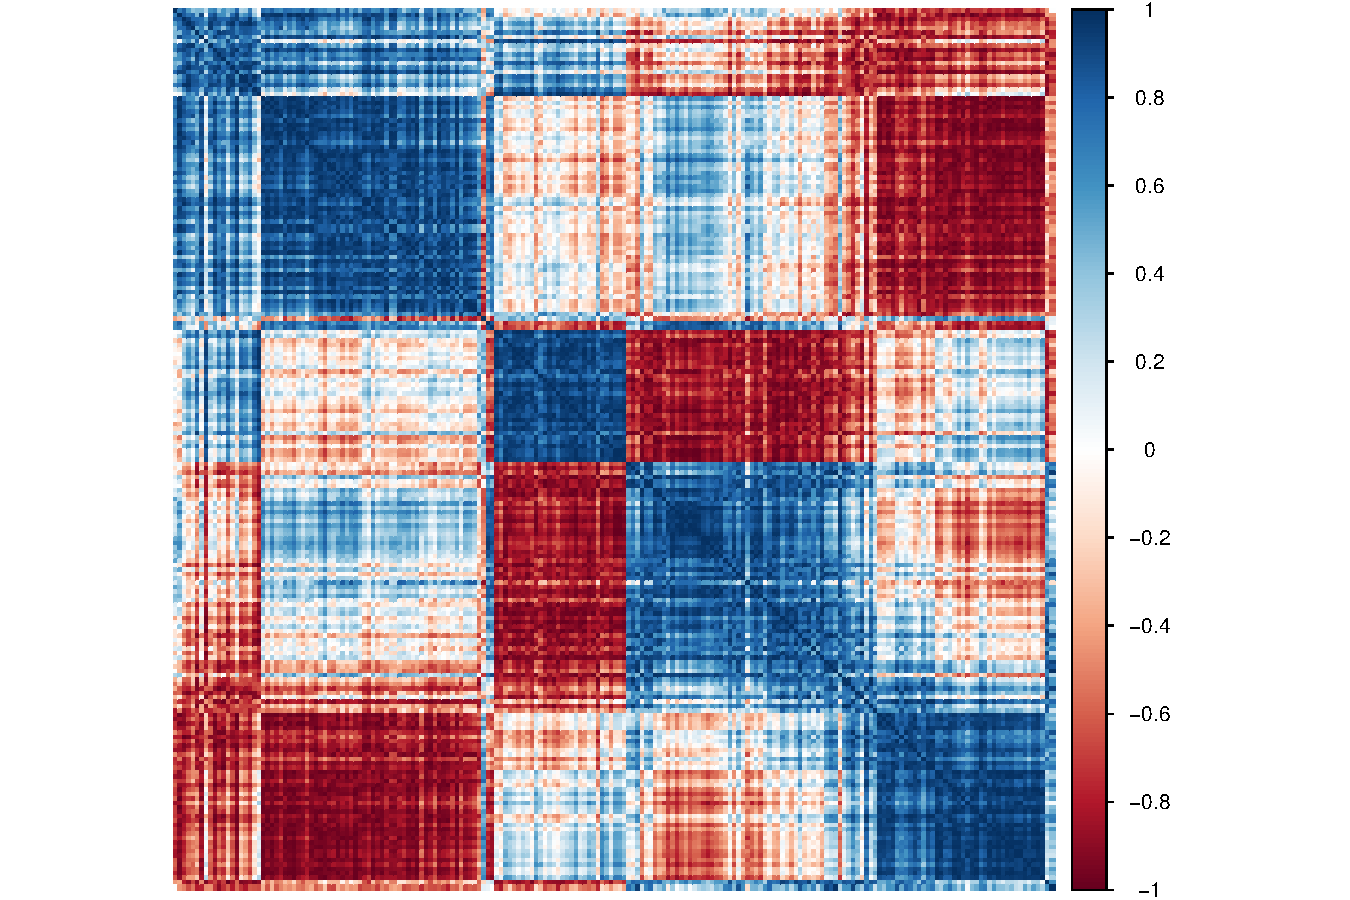
\includegraphics[width=.8\textwidth]{figures/Ward_corrplot-1} 

\end{knitrout}
  

\end{frame}

%% ==========================================================================
\section{Model-based approach}
%% ==========================================================================

\begin{frame}
  \frametitle{References}

    \begin{thebibliography}{99}
      \setbeamertemplate{bibliography item}[book]

    \bibitem[EK2]{EK2} Pattern recognition and machine learning,
    \newblock \textcolor{black}{Christopher Bishop}
    \newblock \alert{Chapter 9: Mixture Models and EM}
    \newblock {\tiny\url{http://users.isr.ist.utl.pt/~wurmd/Livros/school/}}

    \bibitem[SR]{SR} Models with Hidden Structure with Applications in Biology and Genomics,
    \newblock \textcolor{black}{Stéphane Robin}
    \newblock \alert{Master MathSV Course}
    \newblock {\tiny\url{https://www6.inra.fr/mia-paris/content/download/4587/42934/version/1/file/ModelsHiddenStruct-Biology.pdf}}

      \setbeamertemplate{bibliography item}[article]

    \bibitem[CM1]{CM1} Classification non-supervisées,
    \newblock \textcolor{black}{É. Lebarbier, T. Mary-Huard}
    \newblock \alert{Chapitre 3 - méthode probabiliste: le modèle de mélange}
    \newblock {\tiny\url{https://www.agroparistech.fr/IMG/pdf/ClassificationNonSupervisee-AgroParisTech.pdf}}

    \end{thebibliography}


\end{frame}

%% ==========================================================================
\subsection{Mixture models}
%% ==========================================================================

\begin{frame}
  \frametitle{Latent variables models}

  \begin{definition}
    A \alert{latent variable model} is a statistical model that relates, for $i=1,\dots,n$ individuals,
  \begin{itemize}
    \item a set of \alert{manifest} (observed) variables $\bX = (X_i, i=1,\dots,n)$ to
    \item a set of \alert{latent} (unobserved) variables $\bZ = (Z_i, i=1,\dots,n)$.
    \end{itemize}
  \end{definition}

  \begin{block}{Common assumption: conditional independence}
    \vspace{-.5cm}
    \begin{equation*}
      \prob((X_1, \dots, X_n)|(Z_1,\dots, Z_n))  = \prod_{i=1}^n \prob(X_i| Z_i).
    \end{equation*}
  \end{block}

  \vspace{-.25cm}

  \begin{block}{Famous examples}<2->
    \vspace{-.25cm}
    \begin{itemize}
      \item $(Z_i, i\geq 1)$ is Markov chain: \alert{Markov models}
      \item $Z_i$ categorical and independent: \alert{mixture models}
    \end{itemize}
  \end{block}

\end{frame}

\begin{frame}
  \frametitle{Mixture models: the latent variables}

    When $(Z_1,\dots,Z_n)$ are independent categorical variables, they give a \alert{natural (latent) classification of the observations} $(X_1,\dots,X_n)$ -- or \alert{labels}.

  \begin{block}{Notations}<2->
    Let $(Z_1, \dots, Z_n)$ be \textit{iid} categorical variables with distribution
    \vspace{-.25cm}
    \begin{equation*}
      \prob(i \in q) = \prob(Z_i = q) = \alpha_q, \quad \text{s.t.}  \sum_{q=1}^Q \alpha_q = 1.
    \end{equation*}
  \end{block}

  \vspace{-.5cm}
  \begin{block}{Alternative (equivalent) notation}<3>
    Let $Z_i=(Z_{i1},\dots, Z_{iq})$ be an indicator vector of label for $i$:
    \vspace{-.25cm}
    \begin{equation*}
      \prob(i \in q) = \prob(Z_{iq}  =  1)=\alpha_q,  \quad  \text{s.t.} \sum_{q=1}^Q \alpha_q = 1.
    \end{equation*}
    By definition, $Z_i \sim \mathcal{M}(1, \balpha)$, with $\balpha = (\alpha_1, \dots, \alpha_Q)$.
  \end{block}

\end{frame}

\begin{frame}
  \frametitle{Mixture models: the manifest variables}

  A mixture model represents the \alert{presence of subpopulations} within an overall population as follows:
  \begin{equation*}
    \prob(X_i) = \sum_{z_i \in \mathcal{Z}_i} \prob(X_i , Z_i) = \sum_{Z_i \in \mathcal{Z}_i}\prob(X_i | Z_i) \prob(Z_i).
  \end{equation*}

  \vfill

  \begin{block}{Conditional distribution of the manifest variables}
    We assume a \alert{parametric distribution} of $X$ in each subpopulation
    \begin{equation*}
      X_i | \set{Z_i = q} \sim \prob_{\theta_q} \qquad \bigg(\Leftrightarrow X_i | \set{Z_{iq}} = 1 \sim \prob_{\theta_q}\bigg)
    \end{equation*}
    The specificity of each class is handled by $\set{\btheta_q}_{q=1}^Q$.
  \end{block}

\end{frame}

\begin{frame}
  \frametitle{Mixture models: likelihoods}

  \begin{block}{The complete-data likelihood}
    It is the join distribution of $(X_i,Z_i)$:
    \begin{equation*}
      \prob(X_i,Z_i) = \alpha_{Z_i} \prob_{\btheta_{{Z_i}}}(X_i)
    \end{equation*}
  \end{block}

  \vspace{-.25cm}

  \begin{block}{The incomplete-data likelihood}<2>
    It is the marginal distribution of $X_i$ once $Z_i$ integrated:
    \begin{equation*}
      \prob(X_i) = \sum_{q=1}^Q \prob(X_i, Z_i = q)  = \sum_{q=1}^Q \alpha_q \prob_{\btheta_q}(X_i)
    \end{equation*}
  \end{block}

  \vspace{-.25cm}

  \onslide<2>{
    $\rightsquigarrow$ A \alert{mixture model} is a sum of distributions weigthed by the proportion of each subpopulation.
  }

\end{frame}

%% ==========================================================================
\subsection{Expectation-Maximization algorithm}
%% ==========================================================================

\begin{frame}
  \frametitle{Intractability of the Likelihood}

  \begin{block}{Maximum Likelihood Estimator}
    The MLE aims to maximize the (marginal) likehood of the observations:
    \begin{equation*}
      L(\btheta; \bX) = \prob_{\btheta}((X_1,\dots,X_n)) = \int_{\bZ \in \mathcal{Z}} \prob_{\btheta}(\bX,\bZ) \mathrm{d} \bZ
    \end{equation*}
    Integrations are summation over $\set{1,\dots,Q}$: we have $Q^n$ terms !
  \end{block}

  \vfill

  \begin{block}{Intractable summation}<2->
    With mixture models, for $\btheta = (\btheta_1,\dots,\btheta_Q)$ we have
    \begin{equation*}
      \log L(\btheta; \bX) = \sum_{i=1}^n \log \set{\sum_{q=1}^Q \alpha_q \prob_{\btheta_q}(X_i)}.
    \end{equation*}
    \alert{$\rightsquigarrow$ Direct maximization of the likelihood is impossible in practice}
  \end{block}

\end{frame}

\begin{frame}
  \frametitle{Bayes decision rule / Maximum \textit{a posteriori}}

  \begin{block}{Principle}
    Affect an individual $i$ to the subpopulation which is the most likely according to the data:
    \begin{equation*}
      \tau_{iq} = \prob(Z_{iq}=1 | X_i = x_i)
    \end{equation*}
    This is the \alert{posterior probability} for $i\in q$.
  \end{block}

  \vfill

  \begin{block}{Application of the Bayes Theorem}
    It is straightforward to show that
    \begin{equation*}
      \tau_{iq} = \frac{\alpha_q \prob_{\theta_q}(x_i)}{\sum_{q=1}^Q \alpha_q \prob_{\theta_q}(x_i)}
    \end{equation*}
  \end{block}

\end{frame}

\begin{frame}
  \frametitle{Principle of the EM algorithm}

  \begin{block}{If $\btheta$ were known}
    \dots estimating the \alert{posterior probability $\prob(Z_i|\bX)$} of $\bZ$ should be easy\\
    \textit{By means of the Bayes decision rule}
  \end{block}

  \vfill

  \begin{block}{If $\bZ$ were known\dots}
    \dots estimating the \alert{best set of parameter} $\btheta$ should be easy\\
    \textit{This is close to usual maximum likelihood estimation}
  \end{block}

  \vfill

  \begin{block}{EM principle}<2>
    Maximize the marginal likelihood iteratively:
    \begin{enumerate}
      \item Initialize $\btheta$
      \item Compute the probability of $\bZ$ given $\btheta$
      \item Get a better $\btheta$ with the new $\bZ$
      \item Iterate until convergence
    \end{enumerate}
  \end{block}


\end{frame}

\begin{frame}
  \frametitle{Formal algorithm}

  \begin{block}{Initialization: \textcolor{black}{start from a good guess either of $\bZ$ or $\btheta$, then iterate 1-2}}
  \end{block}

  \begin{block}{1. Expectation step}
    Calculate the expected value of the loglikelihood under the current $\btheta$
    \begin{equation*}
      Q\left(\btheta|\btheta^{(t)}\right) = \E_{\bZ|\bX;\btheta^{(t)}}\big[ \log L (\btheta;\bX,\bZ)  \big] \qquad (\textit {needs } \prob_{\btheta^{(t)}}(\bZ|\bX))
    \end{equation*}
  \end{block}

  \vfill

  \begin{block}{2. Maximization step}
    Find the parameters that maximize this quantity
    \begin{equation*}
      \btheta^{(t+1)} = \argmax_{\btheta} Q\left(\btheta|\btheta^{(t)}\right)
    \end{equation*}
  \end{block}

  Stop when $\|\btheta^{(t+1)} - \btheta^{(t)}\| < \varepsilon$ or $\|Q^{(t+1)} - Q^{(t)}\| < \varepsilon$

\end{frame}

\begin{frame}
  \frametitle{(Basic) Convergence analysis}

  \begin{theorem}
    At each step of the EM algorithm, the loglikelihood increases. EM thus reaches a local optimum.
  \end{theorem}

  \begin{proof}
    On board.
  \end{proof}

\end{frame}

\begin{frame}
  \frametitle{Choosing the number of component}

  \begin{block}{Reminder: Bayesian Information Criterion}
    The BIC is a model selection criterion which penalizes the adjustement to the data by the number of parameter in model $\mathcal{M}$ as follows:
    \begin{equation*}
      \mathrm{BIC}(\mathcal{M}) = \log L(\hatbtheta; \bX) - \frac{1}{2}\log(n) \mathrm{df}(\mathcal{M}).
    \end{equation*}
  \end{block}

  \vspace{-.35cm}

  \begin{block}{Integrated Classification Criterion}<2->
    It is an adaptation working with the complete-data likelihood:
    \vspace{-.25cm}
    \begin{align*}
      \mathrm{ICL}(\mathcal{M}) & = \log L(\hatbtheta; \bX, \hat{\bZ}) + \frac{1}{2}\log(n) \mathrm{df}(\mathcal{M}) \\
      & = \mathrm{BIC} - \mathcal{H}(\prob(\hat \bZ | \bX),
    \end{align*}
    where the entropy $\mathcal{H}$ measures the separability of the subpopulations.
  \end{block}

  \vfill

  \onslide<3>{$\rightsquigarrow$ \alert{We choose $\mathcal{M}(Q)$ that maximizes either BIC or ICL}}
\end{frame}

\begin{frame}
  \frametitle{Popular model: Gaussian Multivariate mixture models}

  The distribution of $X_i$ conditional on the label of $i$ is assumed to be a multivariate Gaussian distribution with unknown parameters:
  \begin{equation*}
  X_i | i \in q \sim \mathcal{N}(\bmu_q,\bSigma_q)
  \end{equation*}

  \begin{block}{Complete Likelihood $(\bX,\bZ)$}
  The model complete loglikelihood is
    \begin{multline*}
        \log L(\boldsymbol{\mu},\boldsymbol{\Sigma}; \bX, \bZ)  = \\ \sum_{i=1}^n \sum_{q=1}^Q Z_{iq} \left(\log \alpha_q - \frac{1}{2}\log\mathrm{det}(\bSigma_q) - \frac{1}{2} \|\bx_i - \bmu_q\|^2_{\bSigma_q^{-1}}) \right) + c
   \end{multline*}
  \end{block}
  

  $\rightsquigarrow$ Implementation of the univariate case during the labs.
\end{frame}

% \begin{frame}
%   \frametitle{Mixture of Gaussians}
%   \framesubtitle{Calculs in the univariate case: complete likelihood}
% 
%   The distribution of $X_i$ conditional on the label of $i$ is assumed to be a univariate Gaussian distribution with unknown parameters:
%   \begin{equation*}
%   X_i | Z_{iq} = 1 \sim \mathcal{N}(\mu_q,\sigma^2_q)
%   \end{equation*}
% 
%   \begin{block}{complete Likelihood $(\bX,\bZ)$}
%   The model complete loglikelihood is
%     \begin{multline*}
%         \log L(\boldsymbol{\mu},\boldsymbol{\sigma}^2; \bX, \bZ)  = \\ \sum_{i=1}^n \sum_{q=1}^Q Z_{iq} \left(\log \alpha_q - \log\sigma_q -\log(\sqrt{2\pi}) - \frac{1}{2\sigma_q^2} (x_i - \mu_q)^2 \right)
%    \end{multline*}
%   \end{block}
% 
% \end{frame}

\begin{frame}[fragile,allowframebreaks]
  \frametitle{Gaussian mixture model in \texttt{R}}
  
  The package \texttt{Mclust} is a great reference 
  
  See \url{https://cran.r-project.org/web/packages/mclust/vignettes/mclust.html} 

  
\begin{knitrout}\scriptsize
\definecolor{shadecolor}{rgb}{0.969, 0.969, 0.969}\color{fgcolor}\begin{kframe}
\begin{alltt}
\hlstd{GMM} \hlkwb{<-} \hlstd{crabs_corrected} \hlopt
  \hlkwd{select}\hlstd{(}\hlopt{-}\hlstd{sex,} \hlopt{-}\hlstd{species)} \hlopt
  \hlkwd{Mclust}\hlstd{(}\hlkwc{modelNames} \hlstd{=} \hlkwd{c}\hlstd{(}\hlstr{"EII"}\hlstd{,} \hlstr{"EEI"}\hlstd{))}
\hlkwd{plot}\hlstd{(GMM,} \hlstr{'BIC'}\hlstd{)}
\end{alltt}
\end{kframe}
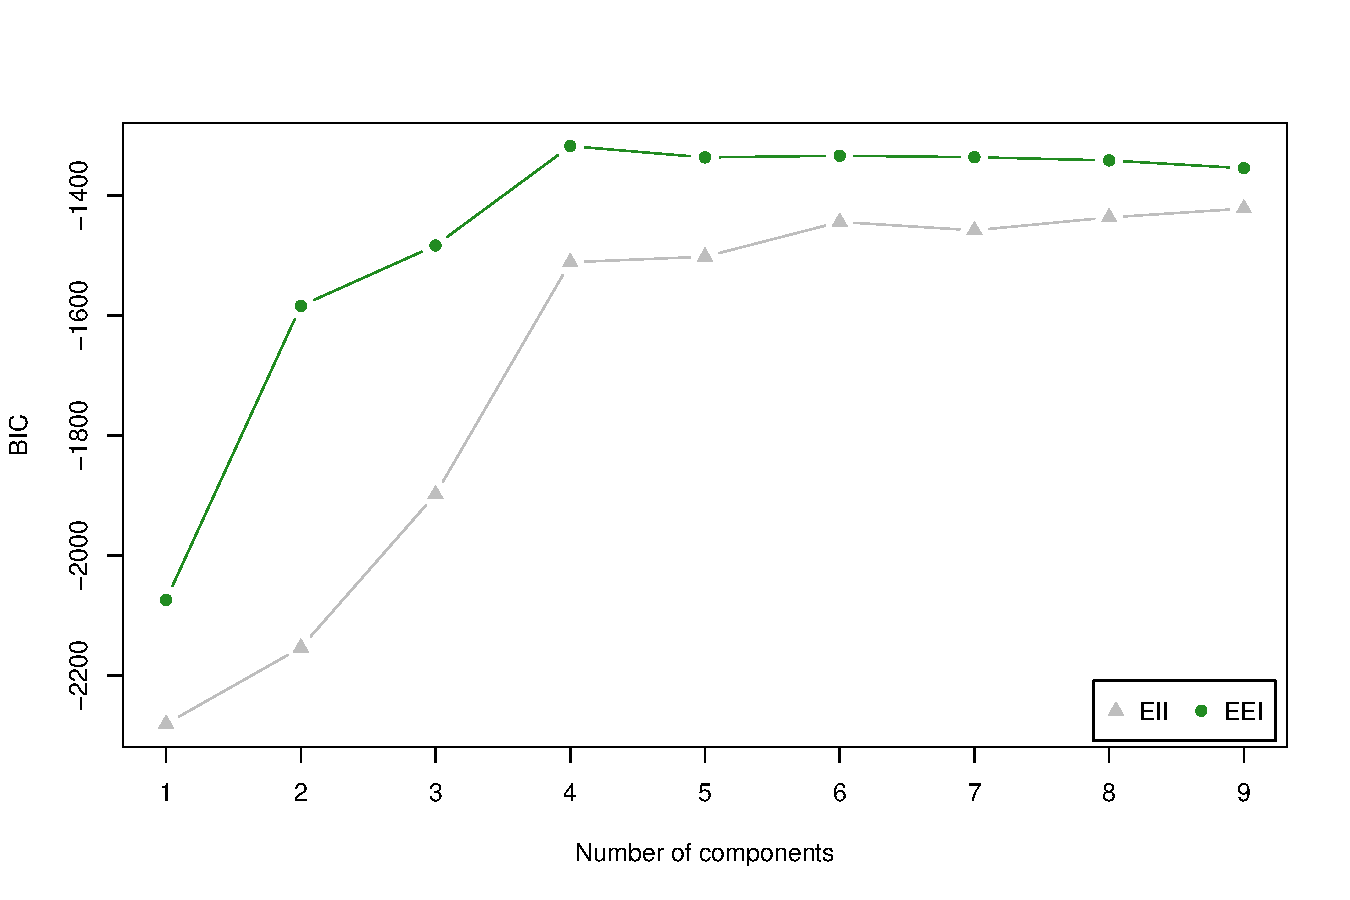
\includegraphics[width=.8\textwidth]{figures/GMM-1} 
\begin{kframe}\begin{alltt}
\hlstd{aricode}\hlopt{::}\hlkwd{ARI}\hlstd{(GMM}\hlopt{$}\hlstd{classification, classes)}
\end{alltt}
\begin{verbatim}
## [1] 0.6451662
\end{verbatim}
\begin{alltt}
\hlstd{aricode}\hlopt{::}\hlkwd{ARI}\hlstd{(GMM}\hlopt{$}\hlstd{classification, clusters)}
\end{alltt}
\begin{verbatim}
## [1] 0.8746812
\end{verbatim}
\begin{alltt}
\hlstd{aricode}\hlopt{::}\hlkwd{ARI}\hlstd{(GMM}\hlopt{$}\hlstd{classification, clusters_ward)}
\end{alltt}
\begin{verbatim}
## [1] 0.8209783
\end{verbatim}
\begin{alltt}
\hlkwd{plot}\hlstd{(GMM,} \hlstr{'classification'}\hlstd{)}
\end{alltt}
\end{kframe}
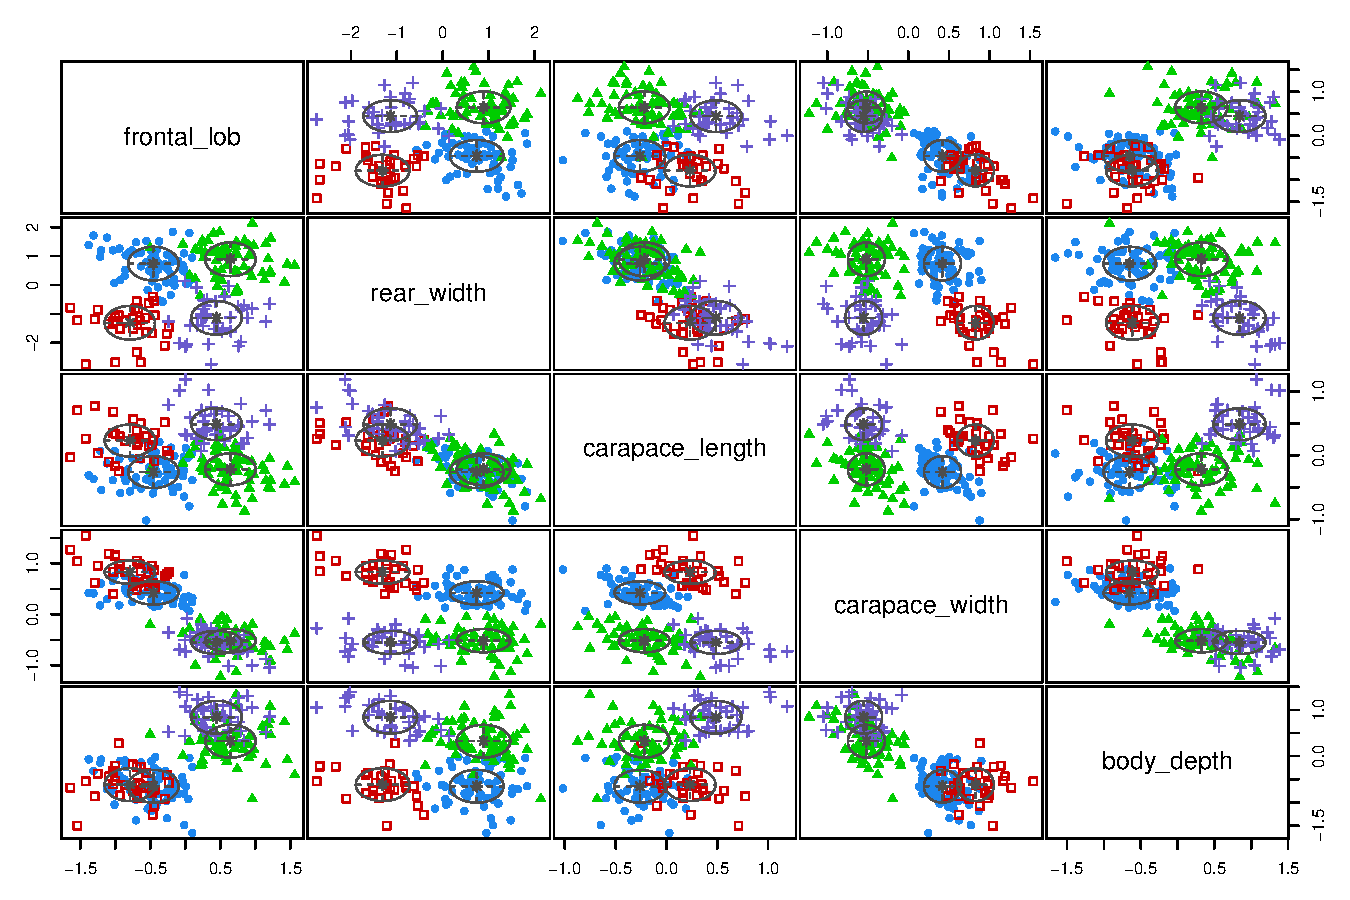
\includegraphics[width=.8\textwidth]{figures/GMM-2} 

\end{knitrout}

\end{frame}


%% ==========================================================================
%% \subsection{Example: mixture of Gaussians}
%% ==========================================================================

% \begin{frame}
%   \frametitle{Mixture of Gaussians}
%   \framesubtitle{Calculs in the univariate case: complete likelihood}
% 
%   The distribution of $X_i$ conditional on the label of $i$ is assumed to be a univariate Gaussian distribution with unknown parameters:
%   \begin{equation*}
%   X_i | Z_{iq} = 1 \sim \mathcal{N}(\mu_q,\sigma^2_q)
%   \end{equation*}
% 
%   \begin{block}{complete Likelihood $(\bX,\bZ)$}
%   The model complete loglikelihood is
%     \begin{multline*}
%         \log L(\boldsymbol{\mu},\boldsymbol{\sigma}^2; \bX, \bZ)  = \\ \sum_{i=1}^n \sum_{q=1}^Q Z_{iq} \left(\log \alpha_q - \log\sigma_q -\log(\sqrt{2\pi}) - \frac{1}{2\sigma_q^2} (x_i - \mu_q)^2 \right)
%    \end{multline*}
%   \end{block}
% 
% \end{frame}
% 
% \begin{frame}
%   \frametitle{Mixture of Gaussians}
%   \framesubtitle{Calculs in the univariate case: E-step}
% 
%   \begin{block}{E-step}
%     For fixed values of  $\mu_q, \sigma_q^2$ and  $\alpha_q$, the  estimates of  the
%   posterior probabilities $\hat\tau_{iq}= \P(Z_{iq}=1|X_i)$ are
%     \begin{equation*}
%         \hat\tau_{iq} = \frac{\alpha_q \mathcal{N}(x_i; {\mu}_q, \sigma_q^2)}{\sum_{q=1}^Q \alpha_q \mathcal{N}(x_i; {\mu}_q, \sigma_q^2)},
%    \end{equation*}
%    where $\mathcal{N}$ is the density of the normal distribution.
%   \end{block}
% 
% \end{frame}
% 
% \begin{frame}
%   \frametitle{Mixture of Gaussians}
%   \framesubtitle{Calculs in the univariate case: M-step}
% 
%   \begin{block}{M-step}
%     For fixed values of  $\tau_{iq}$, the  estimates of  the model parameters are
%     \begin{equation*}
%     \hat\alpha_q = \frac{\sum_{i=1}^n \tau_{iq}}{\sum_{i=1}^n\sum_{q=1}^Q \tau_{iq}} \quad \hat\mu_q = \frac{\sum_i \tau_{iq} x_i}{\sum_i \tau_{iq}} \quad \hat\sigma^2_q = \frac{\sum_{i=1}^n \tau_{iq} (x_i-\mu_q)^2}{\sum_{i=1}^n \tau_{iq}}
%    \end{equation*}
%   \end{block}
% 
% \end{frame}

% \begin{frame}[fragile]
%   \frametitle{R code: auxiliary functions}
% 
% We start by defining functions to compute the complete model loglikelihood, perform the E step and the M step.
% <<EM_mixture_auxiliaries, tidy=FALSE>>=
% get.cloglik <- function(X, Z, theta) {
%   alpha <- theta$alpha; mu <- theta$mu; sigma <- theta$sigma
%   xs <- scale(matrix(X,length(x),length(alpha)),mu,sigma)
%   return(sum(Z*(log(alpha)-log(sigma)-.5*(log(2*pi)+xs^2))))
% }
% 
% M.step <- function(X, tau) {
%   n <- length(X); Q <- ncol(tau)
%   alpha  <- colMeans(tau)
%   mu     <- colMeans(tau * matrix(X,n,Q)) / alpha
%   sigma  <- sqrt(colMeans(tau*sweep(matrix(X,n,Q),2,mu,"-")^2)/alpha)
%   return(list(alpha=alpha, mu=mu, sigma=sigma))
% }
% 
% E.step <- function(X, theta) {
%   tau <- mapply(function(alpha, mu, sigma) {
%       alpha*dnorm(X,mu,sigma)
%     }, theta$alpha, theta$mu, theta$sigma)
%   return(tau / rowSums(tau))
% }
% @
% 
% \end{frame}

% \begin{frame}[fragile]
%   \frametitle{R code: EM for univariate mixture}
% 
% <<EM_mixture, echo=TRUE, tidy=FALSE>>=
% EM.mixture <- function(X, Q,
%                        init.cl=sample(1:Q,n,rep=TRUE), max.iter=100, eps=1e-5) {
%     n <- length(X); tau <- matrix(0,n,Q); tau[cbind(1:n,init.cl)] <- 1
%     Eloglik <- vector("numeric", max.iter)
%     iter <- 0; cond <- FALSE
% 
%     while (!cond) {
%         iter <- iter + 1
%         ## M step
%         theta <- M.step(X, tau)
%         ## E step
%         tau <- E.step(X, theta)
%         ## check consistency
%         Eloglik[iter] <- get.cloglik(X, tau, theta)
%         if (iter > 1)
%             cond <- (iter>=max.iter) | Eloglik[iter]-Eloglik[iter-1] < eps
%     }
% 
%     return(list(alpha = theta$alpha,  mu = theta$mu,  sigma = theta$sigma,
%                 tau   = tau, cl = apply(tau, 1, which.max),
%                 Eloglik = Eloglik[1:iter]))
% }
% @
% \end{frame}

\begin{frame}[fragile]
  \frametitle{Example: data generation}

We first generate data with 4 components:
\begin{knitrout}\scriptsize
\definecolor{shadecolor}{rgb}{0.969, 0.969, 0.969}\color{fgcolor}\begin{kframe}
\begin{alltt}
\hlstd{mu1} \hlkwb{<-} \hlnum{5}   \hlstd{; sigma1} \hlkwb{<-} \hlnum{1}\hlstd{; n1} \hlkwb{<-} \hlnum{100}
\hlstd{mu2} \hlkwb{<-} \hlnum{10}  \hlstd{; sigma2} \hlkwb{<-} \hlnum{1}\hlstd{; n2} \hlkwb{<-} \hlnum{200}
\hlstd{mu3} \hlkwb{<-} \hlnum{15}  \hlstd{; sigma3} \hlkwb{<-} \hlnum{2}\hlstd{; n3} \hlkwb{<-} \hlnum{50}
\hlstd{mu4} \hlkwb{<-} \hlnum{20}  \hlstd{; sigma4} \hlkwb{<-} \hlnum{3}\hlstd{; n4} \hlkwb{<-} \hlnum{100}
\hlstd{cl} \hlkwb{<-} \hlkwd{rep}\hlstd{(}\hlnum{1}\hlopt{:}\hlnum{4}\hlstd{,}\hlkwd{c}\hlstd{(n1,n2,n3,n4))}
\hlstd{x} \hlkwb{<-} \hlkwd{c}\hlstd{(}\hlkwd{rnorm}\hlstd{(n1,mu1,sigma1),}\hlkwd{rnorm}\hlstd{(n2,mu2,sigma2),}
       \hlkwd{rnorm}\hlstd{(n3,mu3,sigma3),}\hlkwd{rnorm}\hlstd{(n4,mu4,sigma4))}
\hlstd{n} \hlkwb{<-} \hlkwd{length}\hlstd{(x)}

\hlcom{## we randomize the class ordering}
\hlstd{rnd} \hlkwb{<-} \hlkwd{sample}\hlstd{(}\hlnum{1}\hlopt{:}\hlstd{n)}
\hlstd{cl} \hlkwb{<-} \hlstd{cl[rnd]}
\hlstd{x}  \hlkwb{<-} \hlstd{x[rnd]}

\hlstd{alpha} \hlkwb{<-} \hlkwd{c}\hlstd{(n1,n2,n3,n4)}\hlopt{/}\hlstd{n}
\end{alltt}
\end{kframe}
\end{knitrout}
\end{frame}

\begin{frame}[fragile, allowframebreaks]
  \frametitle{Example: data generation - plot}

Let us plot the data and the theoretical mixture.
\begin{knitrout}\scriptsize
\definecolor{shadecolor}{rgb}{0.969, 0.969, 0.969}\color{fgcolor}\begin{kframe}
\begin{alltt}
\hlkwd{curve}\hlstd{(alpha[}\hlnum{1}\hlstd{]}\hlopt{*}\hlkwd{dnorm}\hlstd{(x,mu1,sigma1)} \hlopt{+}
      \hlstd{alpha[}\hlnum{2}\hlstd{]}\hlopt{*}\hlkwd{dnorm}\hlstd{(x,mu2,sigma2)} \hlopt{+}
      \hlstd{alpha[}\hlnum{3}\hlstd{]}\hlopt{*}\hlkwd{dnorm}\hlstd{(x,mu3,sigma3)} \hlopt{+}
      \hlstd{alpha[}\hlnum{4}\hlstd{]}\hlopt{*}\hlkwd{dnorm}\hlstd{(x,mu4,sigma4),}
      \hlkwc{col}\hlstd{=}\hlstr{"blue"}\hlstd{,} \hlkwc{lty}\hlstd{=}\hlnum{1}\hlstd{,} \hlkwc{from}\hlstd{=}\hlnum{0}\hlstd{,}\hlkwc{to}\hlstd{=}\hlnum{30}\hlstd{,} \hlkwc{n}\hlstd{=}\hlnum{1000}\hlstd{,}
      \hlkwc{main}\hlstd{=}\hlstr{"Theoretical Gaussian mixture and its components"}\hlstd{,}
      \hlkwc{xlab}\hlstd{=}\hlstr{"x"}\hlstd{,} \hlkwc{ylab}\hlstd{=}\hlstr{"density"}\hlstd{)}
\hlkwd{curve}\hlstd{(alpha[}\hlnum{1}\hlstd{]}\hlopt{*}\hlkwd{dnorm}\hlstd{(x,mu1,sigma1),} \hlkwc{col}\hlstd{=}\hlstr{"red"}\hlstd{,} \hlkwc{add}\hlstd{=}\hlnum{TRUE}\hlstd{,} \hlkwc{lty}\hlstd{=}\hlnum{2}\hlstd{)}
\hlkwd{curve}\hlstd{(alpha[}\hlnum{2}\hlstd{]}\hlopt{*}\hlkwd{dnorm}\hlstd{(x,mu2,sigma2),} \hlkwc{col}\hlstd{=}\hlstr{"red"}\hlstd{,} \hlkwc{add}\hlstd{=}\hlnum{TRUE}\hlstd{,} \hlkwc{lty}\hlstd{=}\hlnum{2}\hlstd{)}
\hlkwd{curve}\hlstd{(alpha[}\hlnum{3}\hlstd{]}\hlopt{*}\hlkwd{dnorm}\hlstd{(x,mu3,sigma3),} \hlkwc{col}\hlstd{=}\hlstr{"red"}\hlstd{,} \hlkwc{add}\hlstd{=}\hlnum{TRUE}\hlstd{,} \hlkwc{lty}\hlstd{=}\hlnum{2}\hlstd{)}
\hlkwd{curve}\hlstd{(alpha[}\hlnum{4}\hlstd{]}\hlopt{*}\hlkwd{dnorm}\hlstd{(x,mu4,sigma4),} \hlkwc{col}\hlstd{=}\hlstr{"red"}\hlstd{,} \hlkwc{add}\hlstd{=}\hlnum{TRUE}\hlstd{,} \hlkwc{lty}\hlstd{=}\hlnum{2}\hlstd{)}
\hlkwd{rug}\hlstd{(x)}
\end{alltt}
\end{kframe}
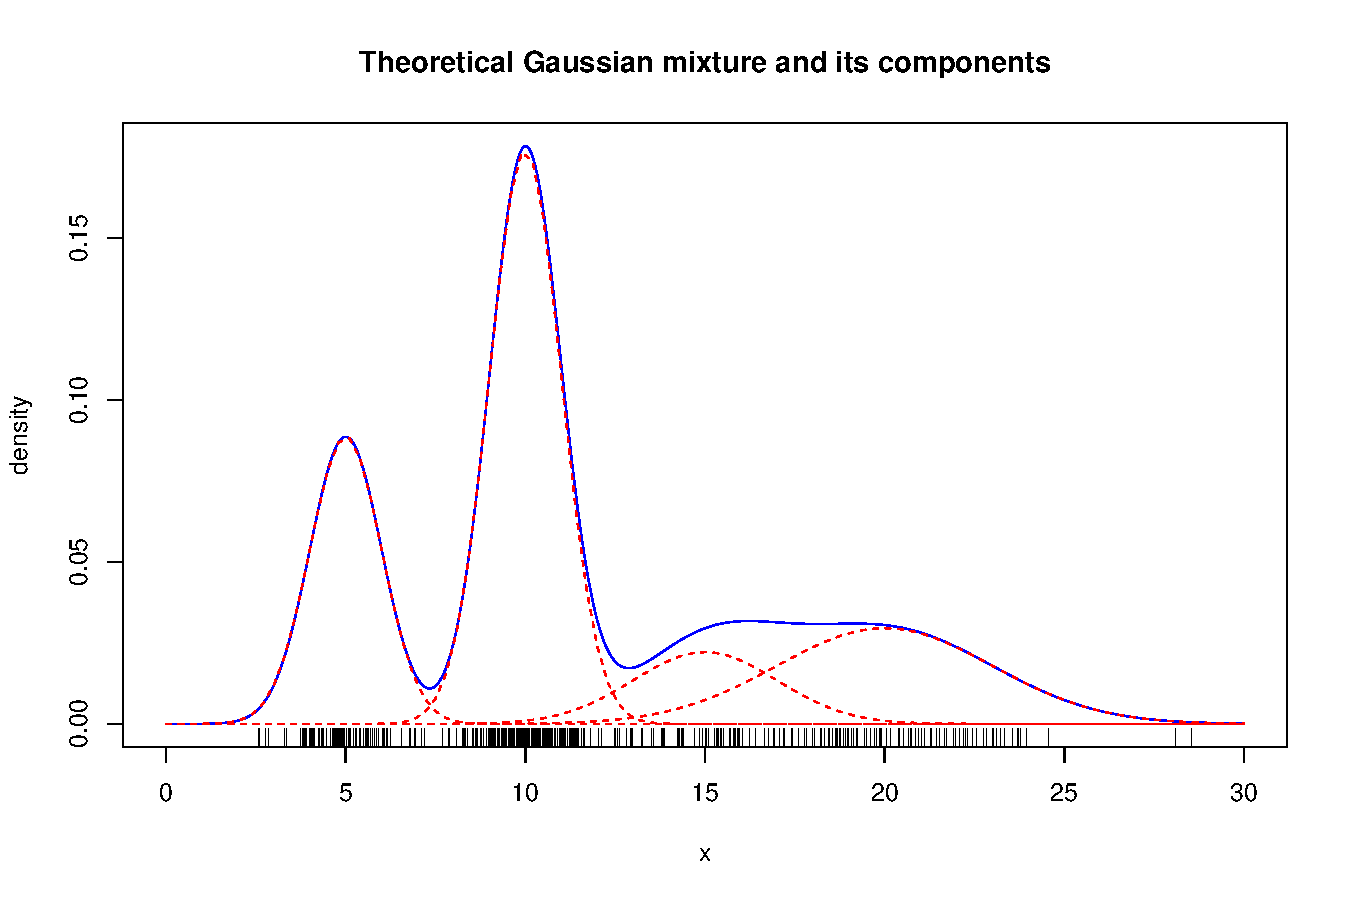
\includegraphics[width=.8\textwidth]{figures/EM_mixture_example_data_plot-1} 

\end{knitrout}
\end{frame}
% 
% \begin{frame}[fragile]
%    \frametitle{Implementation}
%    
%    \begin{center}
%       Your labs!
%    \end{center}
%    
% \end{frame}
% 
% \begin{frame}[fragile]
%   \frametitle{Example: adjustment}
% 
% <<EM_mixture_run>>=
% out <- EM.mixture(x, Q=4, init.cl=sample(1:4,n,rep=TRUE))
% plot(out$Eloglik, main="EM criterion", type="l", xlab="iteration")
% @
% \end{frame}
% 
% \begin{frame}[fragile, allowframebreaks]
%   \frametitle{Example: adjustment - plot}
% 
% <<EM_mixture_run_plot>>=
% out <- EM.mixture(x, Q=4, init.cl=kmeans(x,4)$cl)
% curve(alpha[1]*dnorm(x,mu1,sigma1) +
%       alpha[2]*dnorm(x,mu2,sigma2) +
%       alpha[3]*dnorm(x,mu3,sigma3) +
%       alpha[4]*dnorm(x,mu4,sigma3), col="blue",
%       lty=1, from=0,to=30, n=1000,
%       main="Theoretical Gaussian mixture and estimated components",
%       xlab="x", ylab="density")
% curve(out$alpha[1]*dnorm(x,out$mu[1],out$sigma[1]), col="red", add=TRUE, lty=2)
% curve(out$alpha[2]*dnorm(x,out$mu[2],out$sigma[2]), col="red", add=TRUE, lty=2)
% curve(out$alpha[3]*dnorm(x,out$mu[3],out$sigma[3]), col="red", add=TRUE, lty=2)
% curve(out$alpha[4]*dnorm(x,out$mu[4],out$sigma[4]), col="red", add=TRUE, lty=2)
% rug(x)
% @
% 
% \end{frame}
% 
% \begin{frame}[fragile, allowframebreaks]
%   \frametitle{Example: adjustment - classification}
% 
% <<EM_mixture_run_contingency>>=
% table(cl, out$cl)
% aricode::ARI(cl, out$cl)
% @
% 
% \end{frame}

\end{document}
